\chapter[Proposta]{Proposta}\label{chap:proposta}

Este Capítulo apresenta o projeto prosposto neste trabalho. Aborda primeiro a Seção de \hyperref[sec:contextualizacaop]{Contextualização},
que retoma as \hyperref[sec:questaopesquisa]{Questões de Pesquisa e Desenvolvimento} a serem resolvidas e os desafios envolvendo
Sistemas de Recomendação. Em seguida, apresenta a Seção de \hyperref[sec:poc]{Solução Atual para Sistema de}  
\hyperref[sec:poc]{Recomendação}, que no contexto
da primeira etapa do trabalho, elabora na prática sobre os posśiveis filtros e métodos de \textit{Deep Learning} que podem ser usados
em Sistemas de Recomendação, apresentando as métricas para cada filtro e método usados. Na sequência, apresenta a Seção de
\hyperref[sec:solucao]{Solução Proposta para Sistema de Recomendação}, que com base nos resultados obtidos na Seção 
\hyperref[sec:poc]{Solução Atual para Sistema de Recomendação}, apresenta o modelo a ser utilizado no trabalho, e ideia Inicialmente
para a aplicação. Por fim, têm-se a Seção de \hyperref[sec:resprop]{Resumo do Capítulo}.

\section{Contextualização}\label{sec:contextualizacaop}

A proposta desse trabalho vêm da experiência da autora com recomendações geradas em plataformas de \textit{streaming}, 
percebendo que nem sempre as recomendações eram precisas ou de seu interesse. Dessa forma, voltando para um público mais
geral, levantou-se a questão de como as recomendações influênciavam os usuários dessas plataformas.

Como \mycitetext{acevedo2020plataformas} e \mycitetext{lourencco2021uso} apresentam, os avanços técnologicos e a pandemia do
COVID-19 impulsionaram o uso de serviços de \textit{streaming} nos últimos anos. Nesse contexto, o uso de Sistemas de Recomendação
nas plataformas de \textit{streaming}, induzem o usuário a continuar usando as plataformas de \textit{streaming} 
\cite{HASAN2018220}, contribuindo para o aumento no uso de serviços de \textit{streaming} que vivienciamos.

Porém, como apresentado \mycitetext{7148534}, os atuais Sistemas de Recomendação enfrentam alguns desafios, como 
\textit{Cold Start}, que foram debatidos na Seção de 
\hyperref[sec:contextualizacao]{Contextualização - Capítulo 1 - Introdução}. Esses problemas justificavam as recomendações
imprecisas vivênciadas pela autora. Assim, levantou-se mais uma questão de como poderia-se melhorar a satisfação do usuário
nos Sistemas de Recomendação. Ao cursar a disciplina FGA0083 - APRENDIZADO DE MÁQUINA, no campus do Gama da Universidade de
Brasília, levantou-se uma possível resposta para esta questão. Seria possível utilizar Inteligência Artificial e Aprendizado
de Máquina para incrementar um Sistema de Recomendação.

Dessa forma, esse trabalho se propõe a analisar a satisfação do usuário em um Sistema de Recomendação centrado em Inteligência
Artificial. E para isso, como proposta será desenvolvido um Sistema de Recomendação utilizando Filtros Colaborativos e 
Filtro com Rede Neural Convolucional de \textit{Deep Learning} levantados nas Seções \hyperref[sec:ia]{Inteligência Artificial - Capítulo 2 - Referencial Teórico} e 
\hyperref[sec:filtrodeep]{Filtros baseados em \textit{Deep Learning} - Capítulo 2 - Referencial Teórico}. E em seguida, avaliado
por métricas e por usuários como definido em \hyperref[sec:meteanresul]{Método de Coleta e Análise de Resultados - Capítulo 4 - Metodologia}.

\section{Solução Atual para Sistema de Recomendação}\label{sec:poc}

Existem diversas aplicações de Inteligência Artificial em Sistemas de Recomendação, como levantado nas Seções 
\hyperref[sec:ia]{Inteligência Artificial - Capítulo 2 - Referencial Teórico} e 
\hyperref[sec:filtrodeep]{Filtros Baseados em \textit{Deep Learning} - Capítulo 2 - Referencial Teórico}. A fim de escolher um
modelo para aplicar em um Sistema de Recomendação, foi desenvolvido algumas provas de conceito com os filtros de Inteligência
Articial e as abordagens em \textit{Deep Learning}, e com base nas métricas de avaliação do modelo, por enquanto sem 
validação do usuário, definidas em \hyperref[sec:meteanresul]{Método de Coleta e Análise de Resultados - Capítulo 4 - Metodologia}, 
foi escolhido o modelo a ser usado na proposta. 
Para a escolha dos Filtros, embora a literatura aponte os Filtros Híbridos
como melhor abordagem, como defendido na Sub Seção \hyperref[subsec:hibridos]{Filtros Híbridos - Capítulo 2 - Referencial Teórico},
o modelo de filtragem híbrida, utilizando Filtro Colaborativo e Filtro de Conteúdo, durante o seu treinamento no Colab 
\cite{colabsite} apresentou problemas de memória no Filtro de Conteúdo, encerrando
a execução antes de finalizar o treinamento. Por essa razão, o filtro a ser utilizado será Filtro Colaborativo. Já para a 
abordagem de \textit{Deep Learning} a ser utilizada em cima do filtro escolhido, com base nas provas de conceito a serem abordadas
nas próximas seções, foi escolhida a com melhores métricas: a abordagem de Rede Neural Convolucional.

Ainda para a elaboração das abordagens de \textit{Deep Learning}, foi feito alguns testes com Máquina Restrita de Boltzmann,
mas não foi possível chegar a um modelo treinado que tivesse resultados satisfatórios, por isso para a escolha dos
Filtros Baseados em \textit{Deep Learning} levou-se em consideração apenas Rede Neural Convolucional, Rede Neural Recorrente,
e Autoencoder.

Para treinar os modelos de Sistema de Recomendação, foi escolhido a base de dados do \mycitetext{parashar2023}
de filmes, como abordado na Sub Seção do \hyperref[subsec:kaggle]{Kaggle - } \hyperref[subsec:kaggle]{Suporte Tecnológico}. 
Esta, possui em sua estrutura um identificador único para usuários (\textit{userId}) e para filmes (\textit{movieId}); 
a avaliação que o usuário deu para o filme (\textit{ratings}); o horário que ocorreu a avaliação do filme 
\textit{timestamp}; o título do filme (\textit{title}), e os gêneros do filme (\textit{genres}). 
Como demonstrado na Figura \hyperref[fig:base]{17}:
\begin{figure}[htbp]
    \centering
    \caption{Base de Dados}
    \label{fig:base}
    
    \vspace{2pt} % Espaço vertical entre a legenda e a imagem
    
    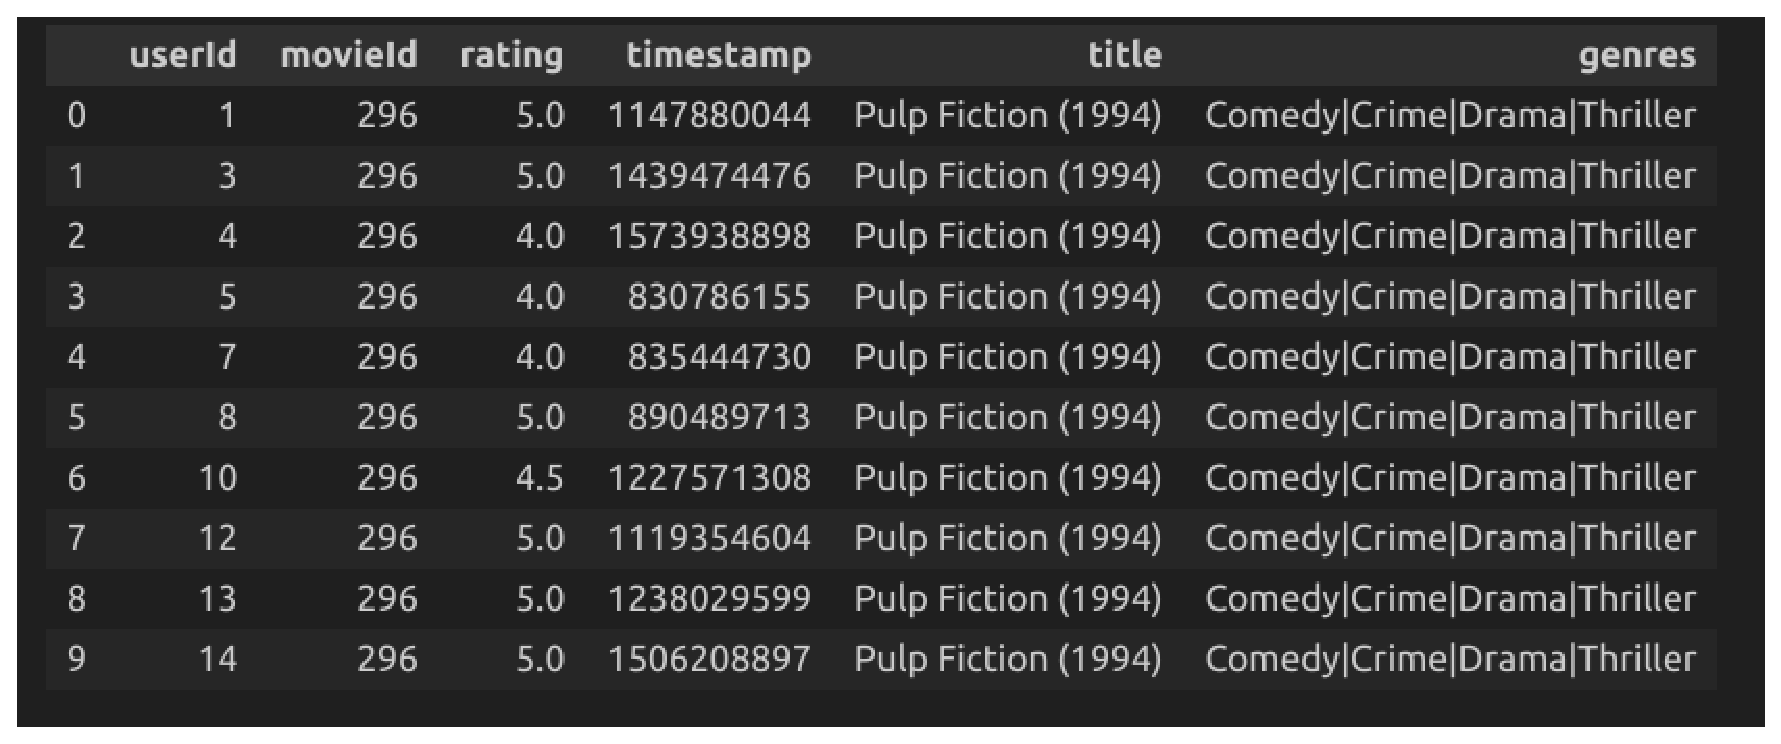
\includegraphics[width=0.5\textwidth]{figuras/base.eps}
    
    \vspace{2pt} % Espaço vertical entre a imagem e a fonte da imagem
    
    \small Fonte: Autora
\end{figure}

\subsection{Modelo com Filtros Colaborativos}\label{subsec:fcolab}

Antes de treinar o modelo com as abordagem de \textit{Deep Learning}, no contexto desse trabalho, é preciso ter uma base com 
um filtro de Inteligência Articial que se aplica a Sistemas de Recomendação. Para isso, foi escolhido o Filtro Colaborativo,
por consumir menos memória durante a execução.

Utilizando a linguagem python, foi criada uma classe para os Filtros Colaborativos, separada em três funções principais 
(funções que executam toda as lógicas principais do modelo, sendo estas treinar, avaliar e recomendar) e três
auxiliares (funções que para quesito de organização foram separadas do código principal, apresentam alguma lógica 
importante na elaboração do código e por isso merecem destaque), sendo elas:

\begin{itemize}
    \item Preparar Dados: Função auxiliar, responsável por carregar os dados da base de dados e separar as colunas a serem 
    utilizadas. Apresentado na Figura \hyperref[fig:prepdata-fc]{18};
    \begin{figure}[htbp]
        \centering
        \caption{Preparar Dados - Filtro Colaborativo}
        \label{fig:prepdata-fc}
        
        \vspace{2pt} % Espaço vertical entre a legenda e a imagem
        
        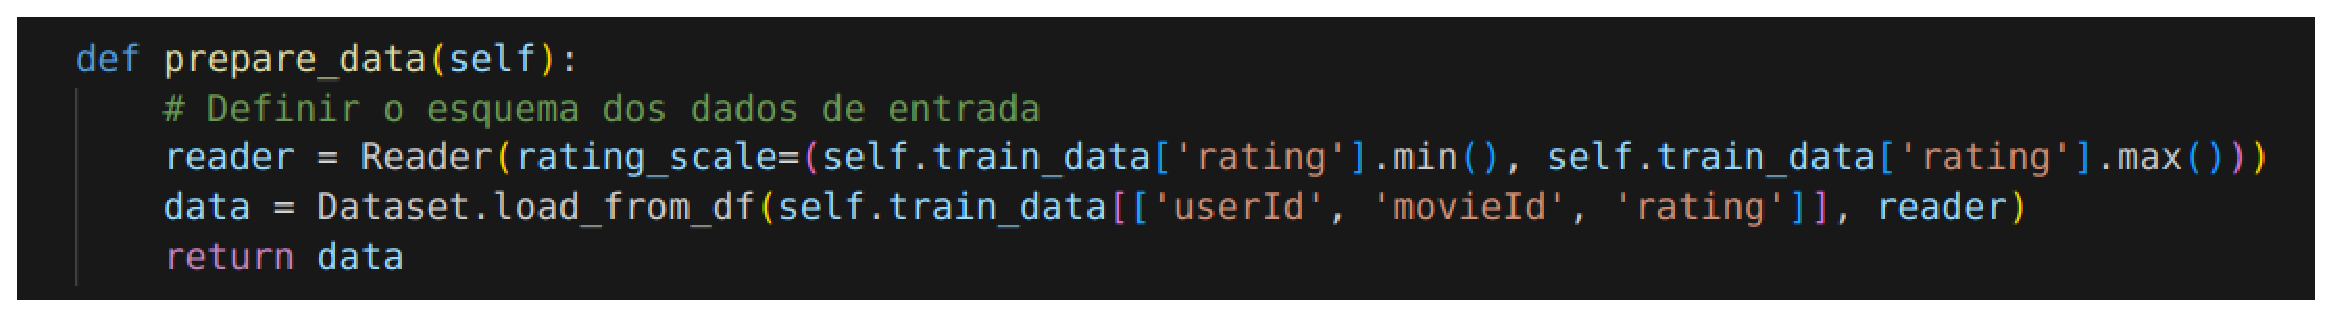
\includegraphics[width=0.5\textwidth]{figuras/prepdata-fc.eps}
        
        \vspace{2pt} % Espaço vertical entre a imagem e a fonte da imagem
        
        \small Fonte: Autora
    \end{figure}

    \item Treinar Modelo: Função principal, responsável por treinar o modelo. Apresentado na Figura \hyperref[fig:train-fc]{19};
    \begin{figure}[htbp]
        \centering
        \caption{Treinar Modelo - Filtro Colaborativo}
        \label{fig:train-fc}
        
        \vspace{2pt} % Espaço vertical entre a legenda e a imagem
        
        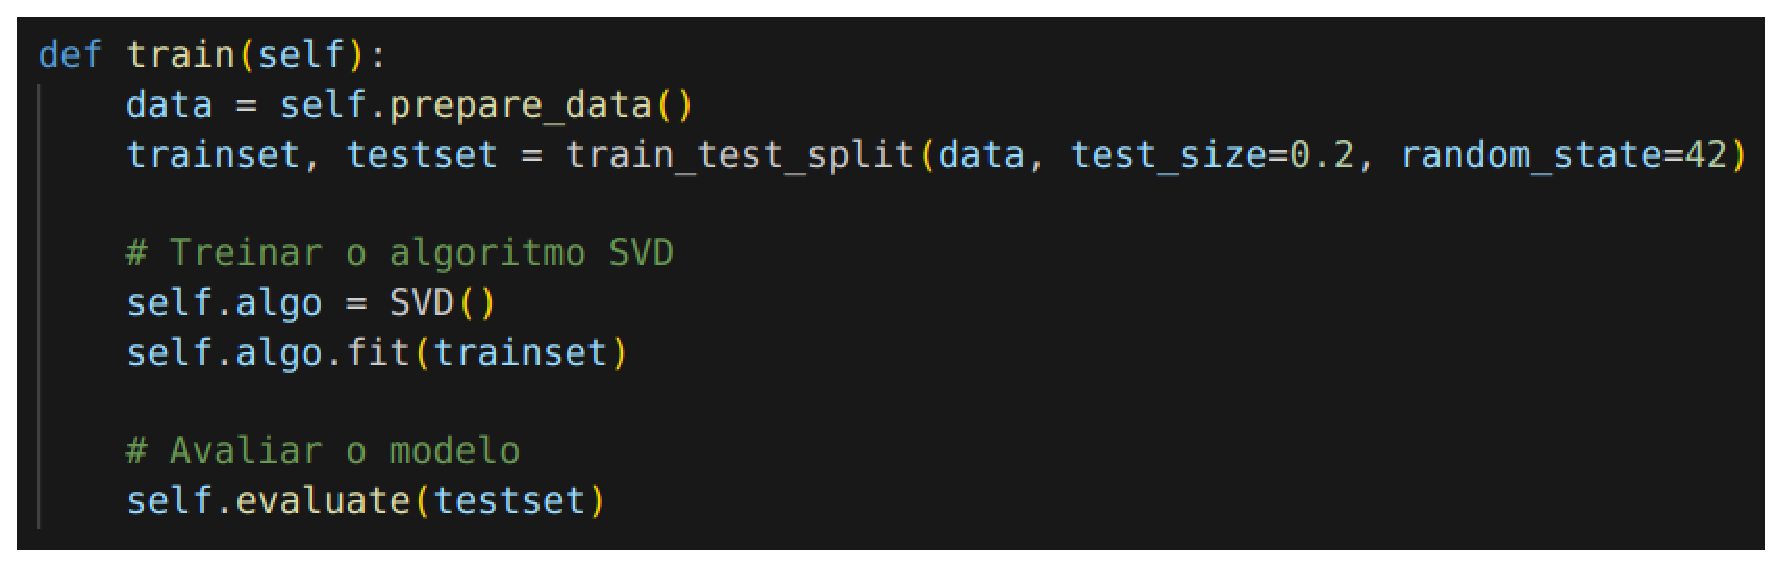
\includegraphics[width=0.5\textwidth]{figuras/train-fc.eps}
        
        \vspace{2pt} % Espaço vertical entre a imagem e a fonte da imagem
        
        \small Fonte: Autora
    \end{figure}

    \item Avaliar Modelo: Função principal, responsável por avaliar o modelo com base nas métricas definidas na Seção 
    \hyperref[sec:meteanresul]{Método de Coleta e Análise de Resultados - Capítulo 4}
    \hyperref[sec:meteanresul]{ - Metodologia} 
    (Precisão, Revocação, Erro Médio Absoluto, Erro Quadrático Médio da Raiz).
    Apresentado na Figura \hyperref[fig:evaluate-fc]{20};
    \begin{figure}[htbp]
        \centering
        \caption{Avaliar Modelo - Filtro Colaborativo}
        \label{fig:evaluate-fc}
        
        \vspace{2pt} % Espaço vertical entre a legenda e a imagem
        
        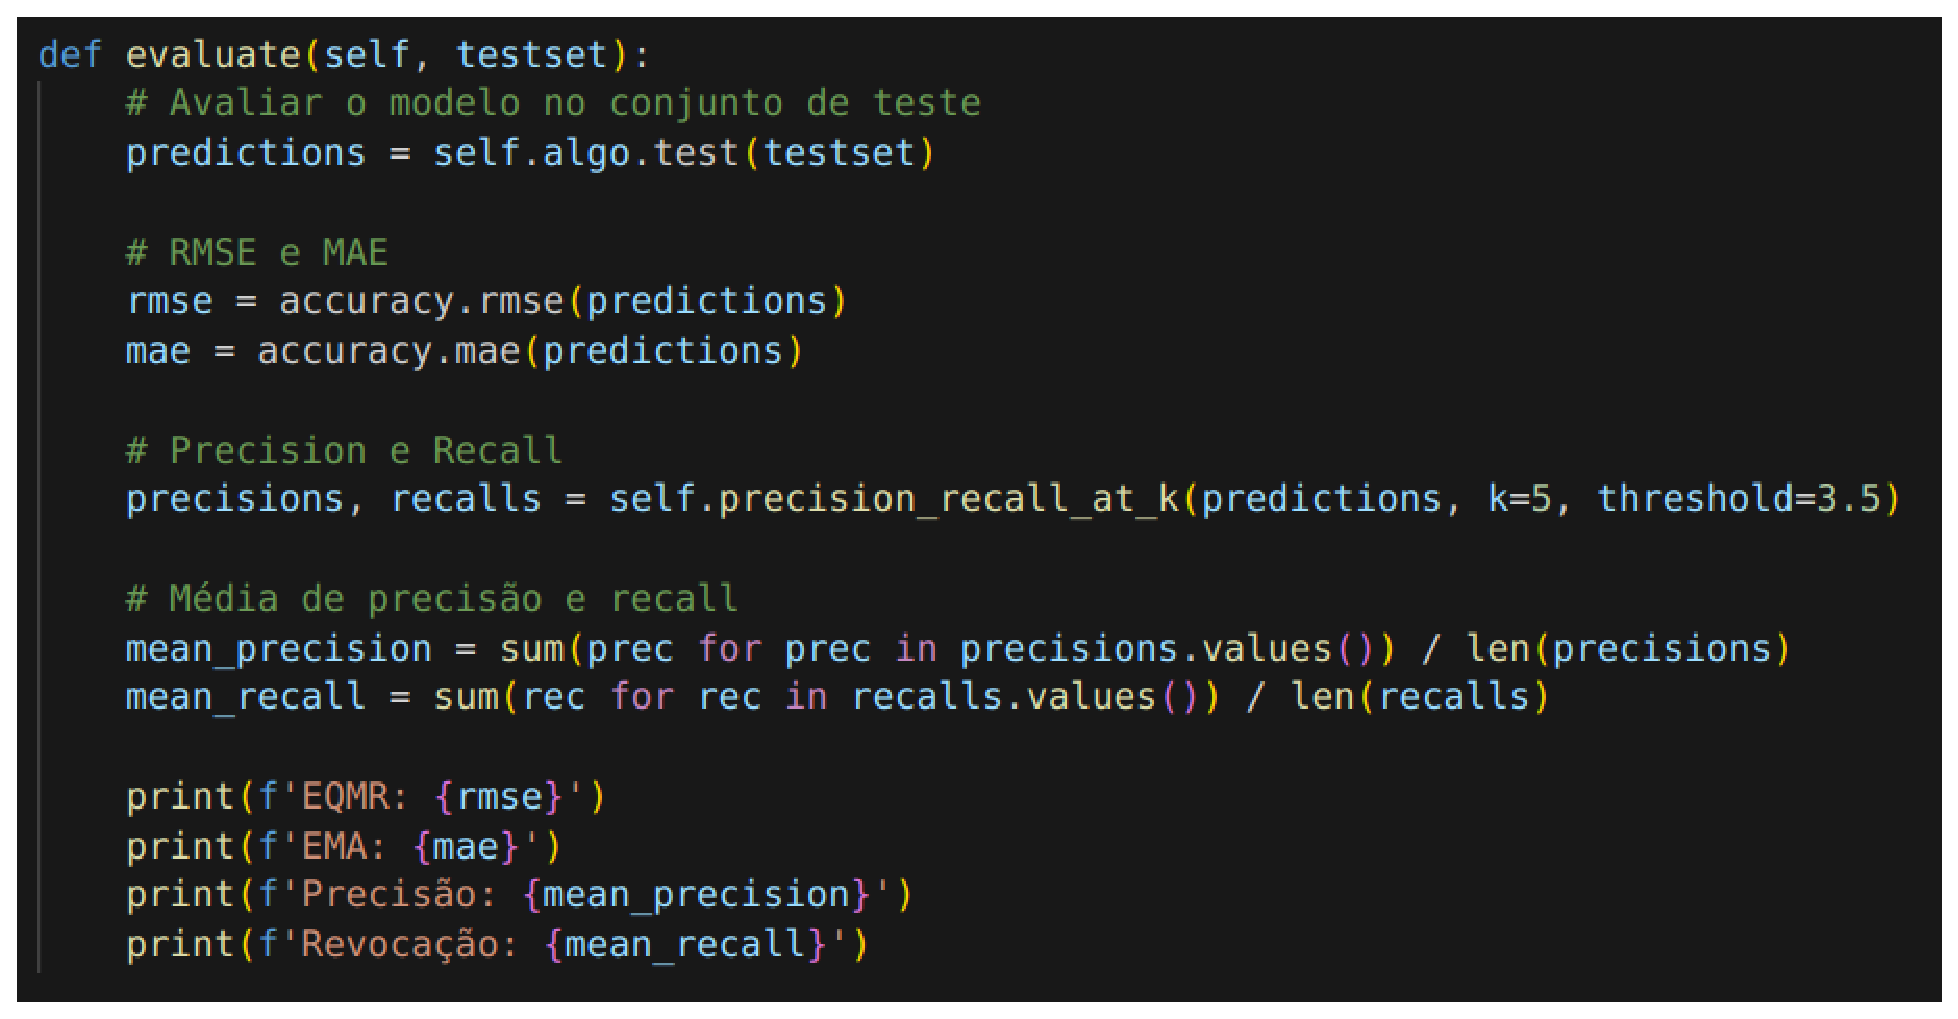
\includegraphics[width=0.5\textwidth]{figuras/evaluate-fc.eps}
        
        \vspace{2pt} % Espaço vertical entre a imagem e a fonte da imagem
        
        \small Fonte: Autora
    \end{figure}

    \item Calcular Precisão e Revocação: Função auxiliar, responsável por calcular a Precisão e Revocação do modelo.
    Apresentado na Figura \hyperref[fig:calc-prec-fc]{21};
    \begin{figure}[htbp]
        \centering
        \caption{Avaliar Modelo - Filtro Colaborativo}
        \label{fig:calc-prec-fc}
        
        \vspace{2pt} % Espaço vertical entre a legenda e a imagem
        
        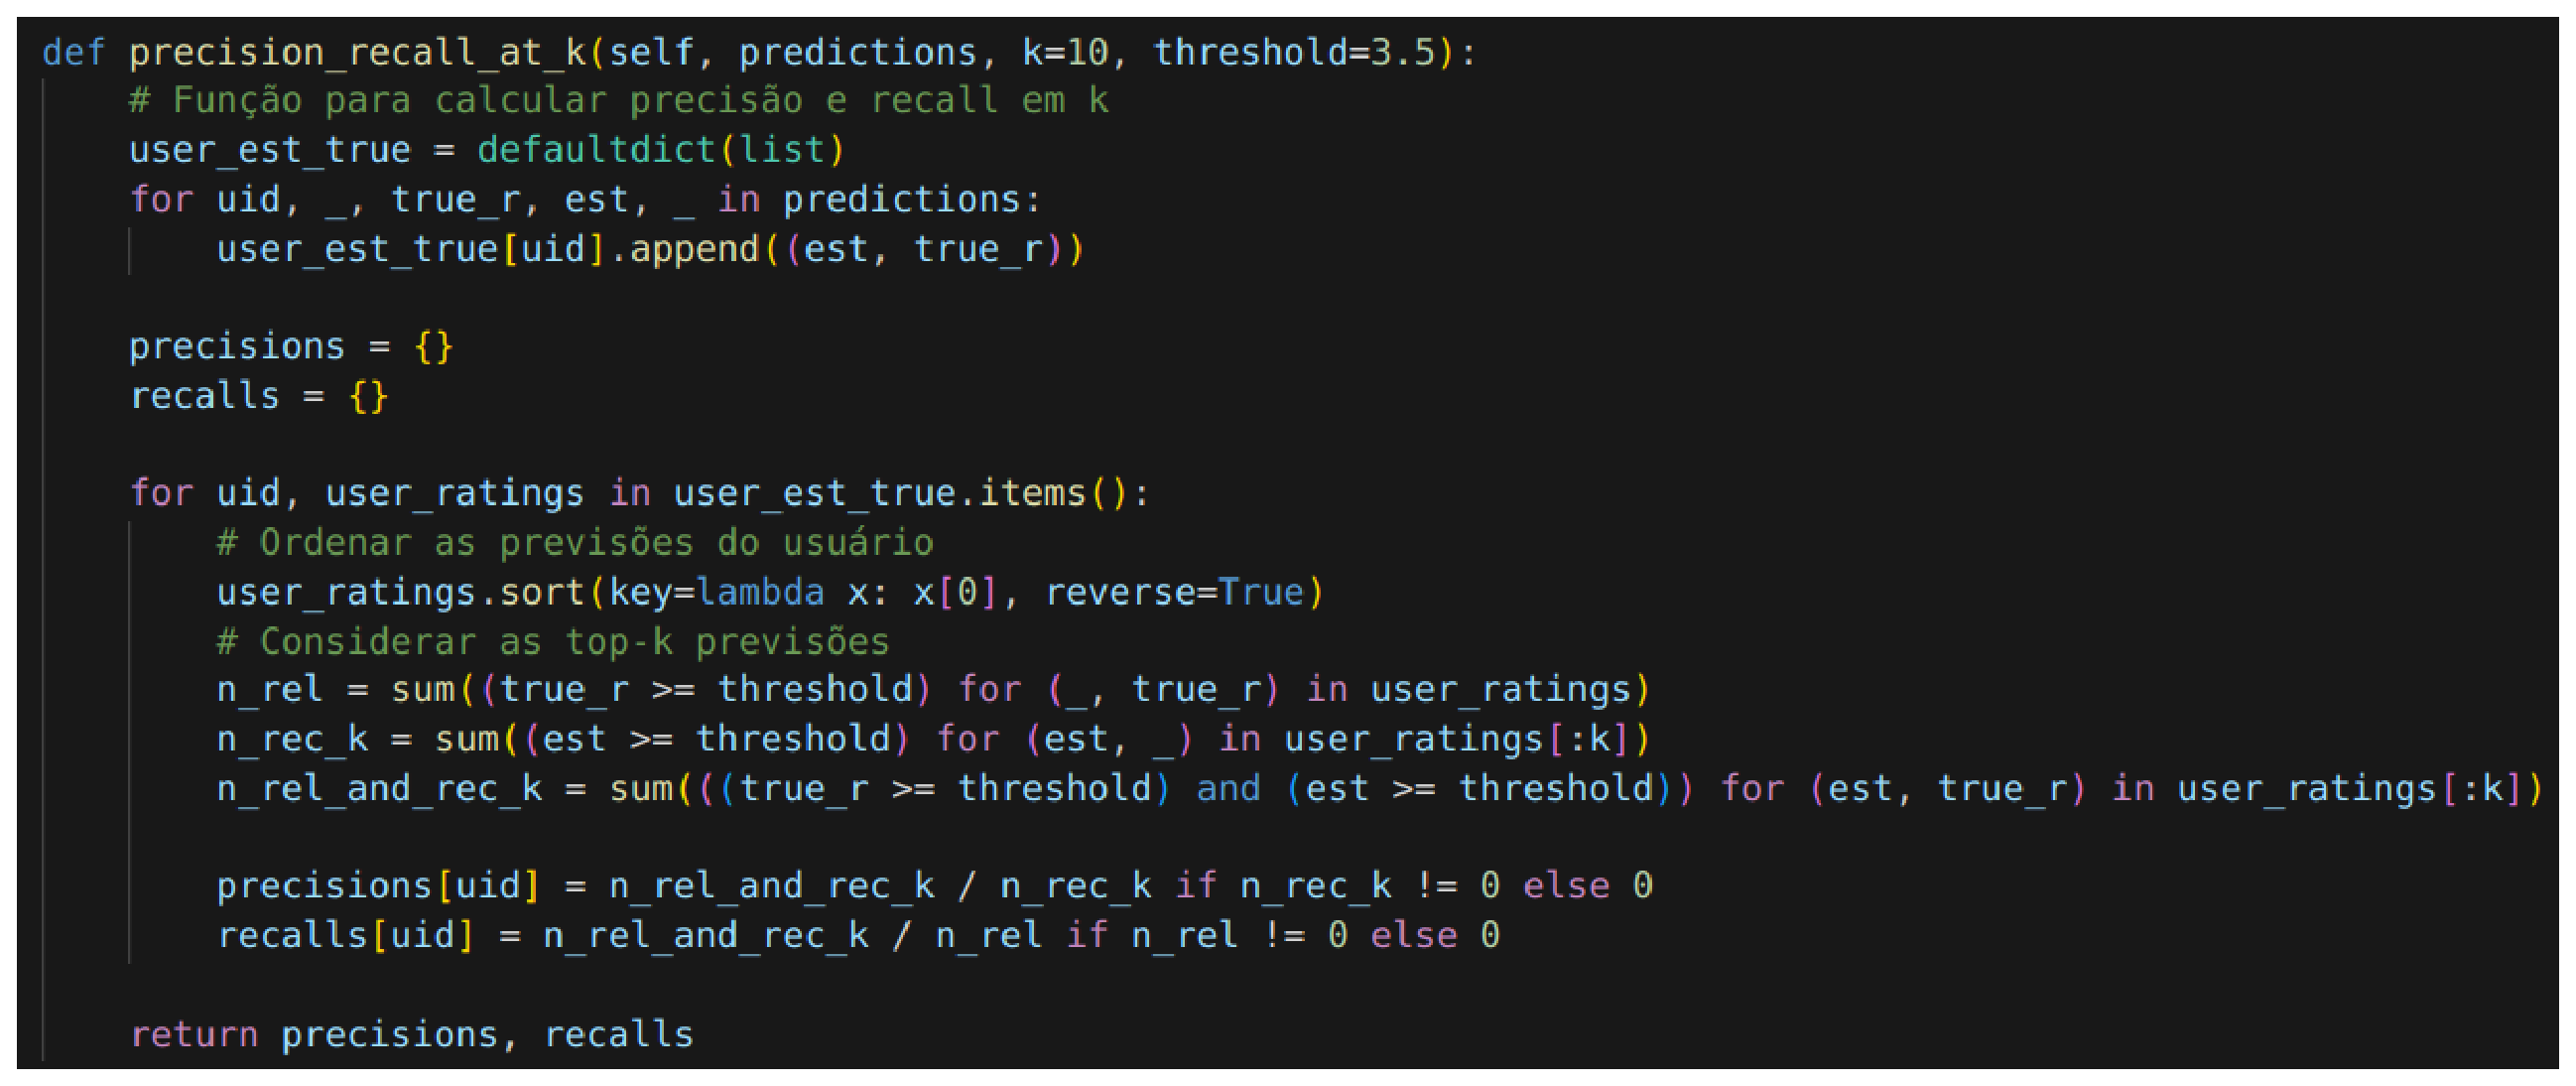
\includegraphics[width=0.5\textwidth]{figuras/calc-prec-fc.eps}
        
        \vspace{2pt} % Espaço vertical entre a imagem e a fonte da imagem
        
        \small Fonte: Autora
    \end{figure}

    \item Prever Avaliação: Função auxiliar, responsável por prever a avaliação do usuário para os filmes.
    Apresentado na Figura \hyperref[fig:prev-fc]{22}, e
    \begin{figure}[htbp]
        \centering
        \caption{Prever Avaliação - Filtro Colaborativo}
        \label{fig:prev-fc}
        
        \vspace{2pt} % Espaço vertical entre a legenda e a imagem
        
        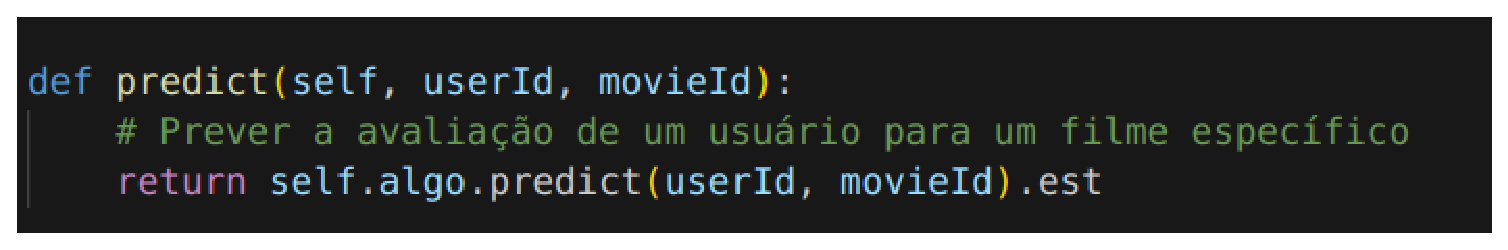
\includegraphics[width=0.5\textwidth]{figuras/prev-fc.eps}
        
        \vspace{2pt} % Espaço vertical entre a imagem e a fonte da imagem
        
        \small Fonte: Autora
    \end{figure}

    \item Obter Recomendação: Função principal, responsável por recomendar ao usuário um filme.
    Apresentado na Figura \hyperref[fig:recom-fc]{23}.
    \begin{figure}[htbp]
        \centering
        \caption{Obter Recomendação - Filtro Colaborativo}
        \label{fig:recom-fc}
        
        \vspace{2pt} % Espaço vertical entre a legenda e a imagem
        
        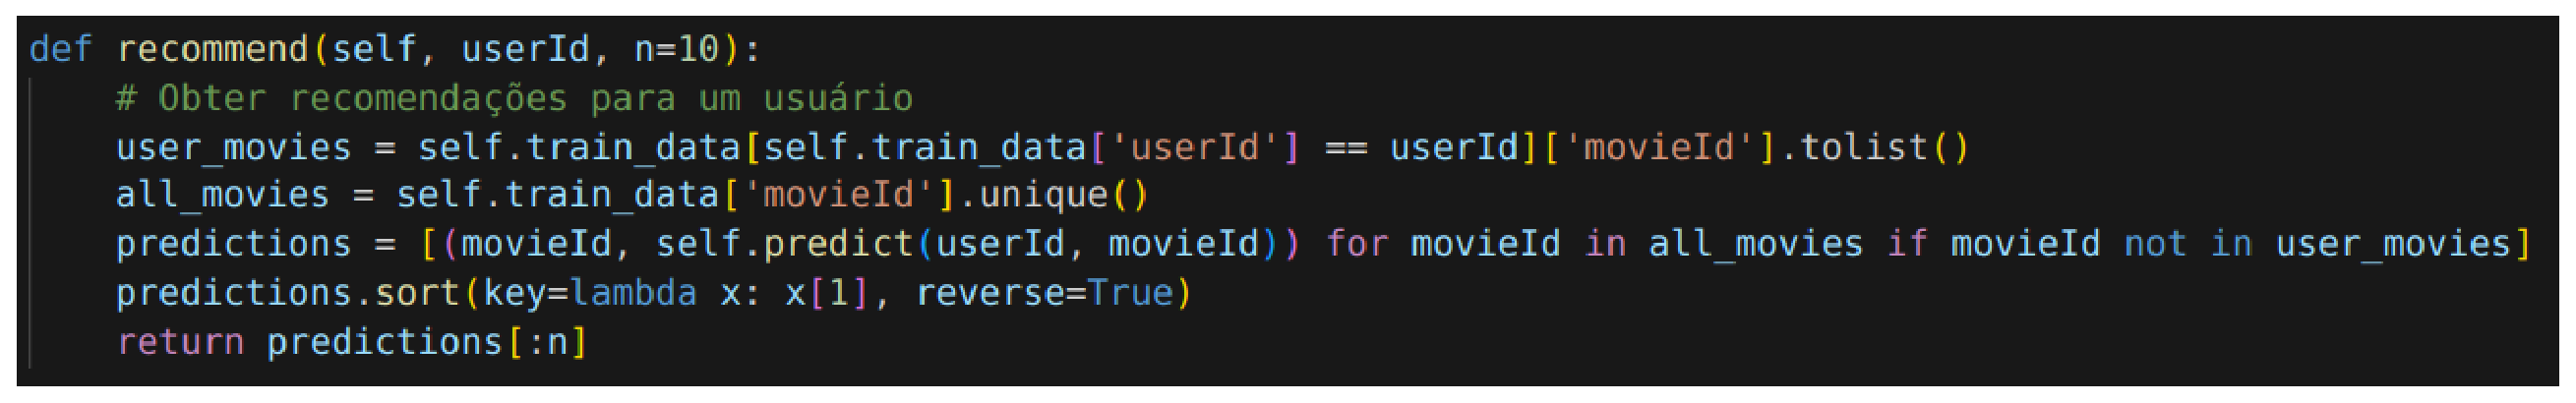
\includegraphics[width=0.5\textwidth]{figuras/recom-fc.eps}
        
        \vspace{2pt} % Espaço vertical entre a imagem e a fonte da imagem
        
        \small Fonte: Autora
    \end{figure}

\end{itemize}

Com essa classe definida, foram realizadas alguns testes alterando o tamanho da base de dados, para entender
as diferenças que uma base bem definida tem no modelo. Foi obtido os seguintes resultados:

\begin{itemize}
    \item Utilizando 5\%\ da Base mostrado na Figura \hyperref[fig:fc-5]{24}:
    \begin{figure}[htbp]
        \centering
        \caption{5\%\ da Base - Filtro Colaborativo}
        \label{fig:fc-5}
        
        \vspace{2pt} % Espaço vertical entre a legenda e a imagem
        
        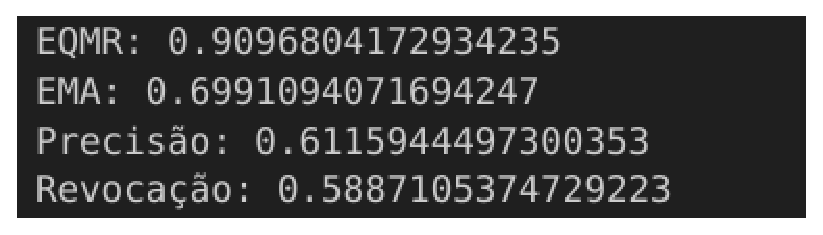
\includegraphics[width=0.5\textwidth]{figuras/fc-5.eps}
        
        \vspace{2pt} % Espaço vertical entre a imagem e a fonte da imagem
        
        \small Fonte: Autora
    \end{figure}

    \item Utilizando 40\%\ da Base mostrado na Figura \hyperref[fig:fc-40]{25}:
    \begin{figure}[htbp]
        \centering
        \caption{40\%\ da Base - Filtro Colaborativo}
        \label{fig:fc-40}
        
        \vspace{2pt} % Espaço vertical entre a legenda e a imagem
        
        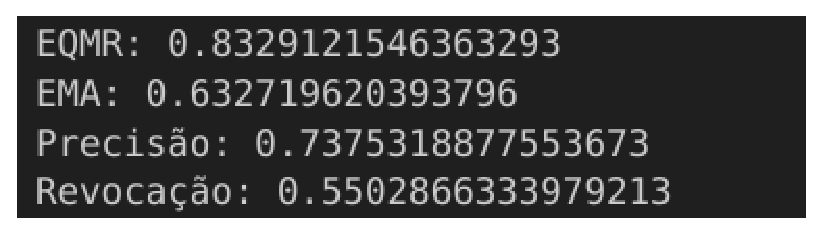
\includegraphics[width=0.5\textwidth]{figuras/fc-40.eps}
        
        \vspace{2pt} % Espaço vertical entre a imagem e a fonte da imagem
        
        \small Fonte: Autora
    \end{figure}

    \item Utiliazando 100\%\ da Base mostrado na Figura \hyperref[fig:fc-100]{26}:
    \begin{figure}[htbp]
        \centering
        \caption{100\%\ da Base - Filtro Colaborativo}
        \label{fig:fc-100}
        
        \vspace{2pt} % Espaço vertical entre a legenda e a imagem
        
        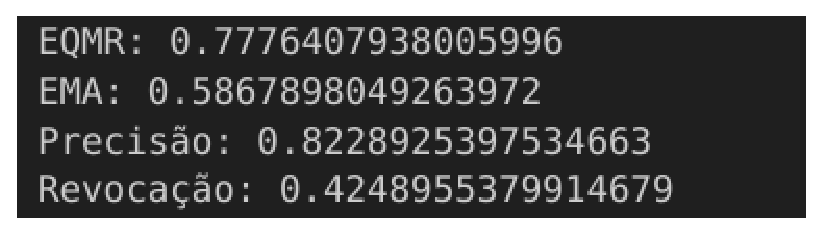
\includegraphics[width=0.5\textwidth]{figuras/fc-100.eps}
        
        \vspace{2pt} % Espaço vertical entre a imagem e a fonte da imagem
        
        \small Fonte: Autora
    \end{figure} 

\end{itemize}

Podemos observar que ao aumentar a base, os parâmetros de Erro Médio Absoluto e Erro Quadrático Médio da Raiz diminuem,
e os parâmetros de Precisão e Revocação aumentam. Indicando que quanto maior a quantidade de dados disponíveis para
treinar o modelo, melhor será sem desempenho.

\subsection{Modelo com Redes Neurais Convolucionais}\label{subsec:rnc}

Usando como base o modelo de Filtros Colaborativos, por questão de memória do servidor do Colab, optou-se pela
versão que utiliza 5\%\ da base de dados.

Similar ao que foi feito para os Filtros Colaborativos, foi criado uma classe de Redes Neurais Convolucionais, com as mesmas
três funções principais (treinar, avaliar e recomendar), porém com apenas duas funções auxiliares, sendo elas:

\begin{itemize}
    \item Preparar Dados: Função auxiliar, responsável por carregar os dados da base de dados e separar as colunas a serem 
    utilizadas. Apresentado na Figura \hyperref[fig:prep-dados-cnn]{27};
    \begin{figure}[htbp]
        \centering
        \caption{Preparar Dados - Rede Neural Convolucional}
        \label{fig:prep-dados-cnn}
        
        \vspace{2pt} % Espaço vertical entre a legenda e a imagem
        
        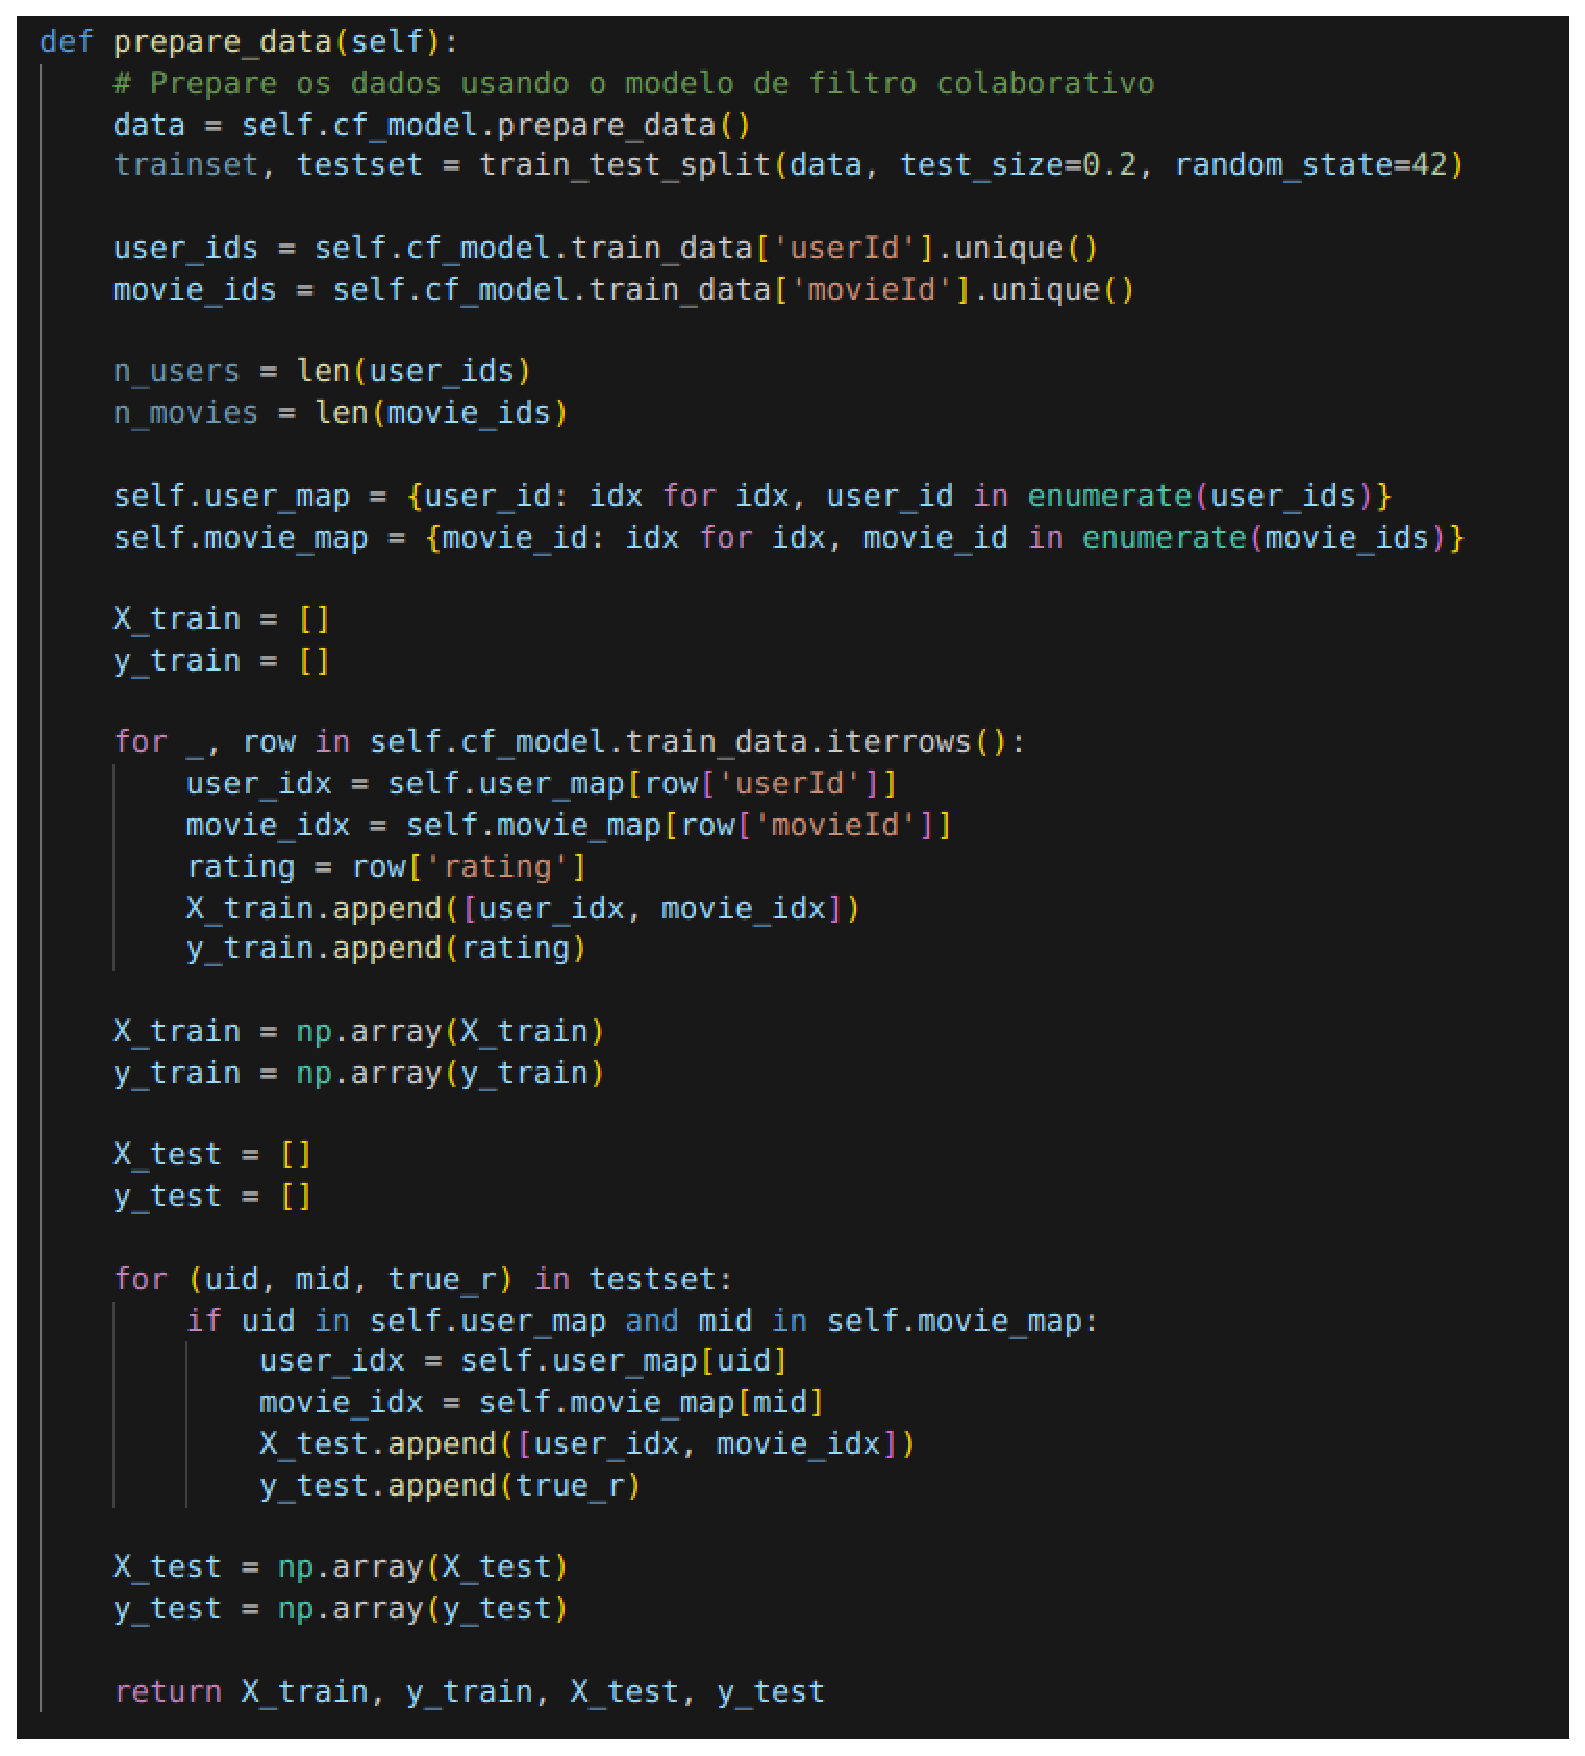
\includegraphics[width=0.5\textwidth]{figuras/prep-dados-cnn.eps}
        
        \vspace{2pt} % Espaço vertical entre a imagem e a fonte da imagem
        
        \small Fonte: Autora
    \end{figure}

    \item Treinar Modelo: Função principal, responsável por treinar o modelo. Apresentado na Figura \hyperref[fig:train-cnn]{28};
    \begin{figure}[htbp]
        \centering
        \caption{Treinar Modelo - Rede Neural Convolucional}
        \label{fig:train-cnn}
        
        \vspace{2pt} % Espaço vertical entre a legenda e a imagem
        
        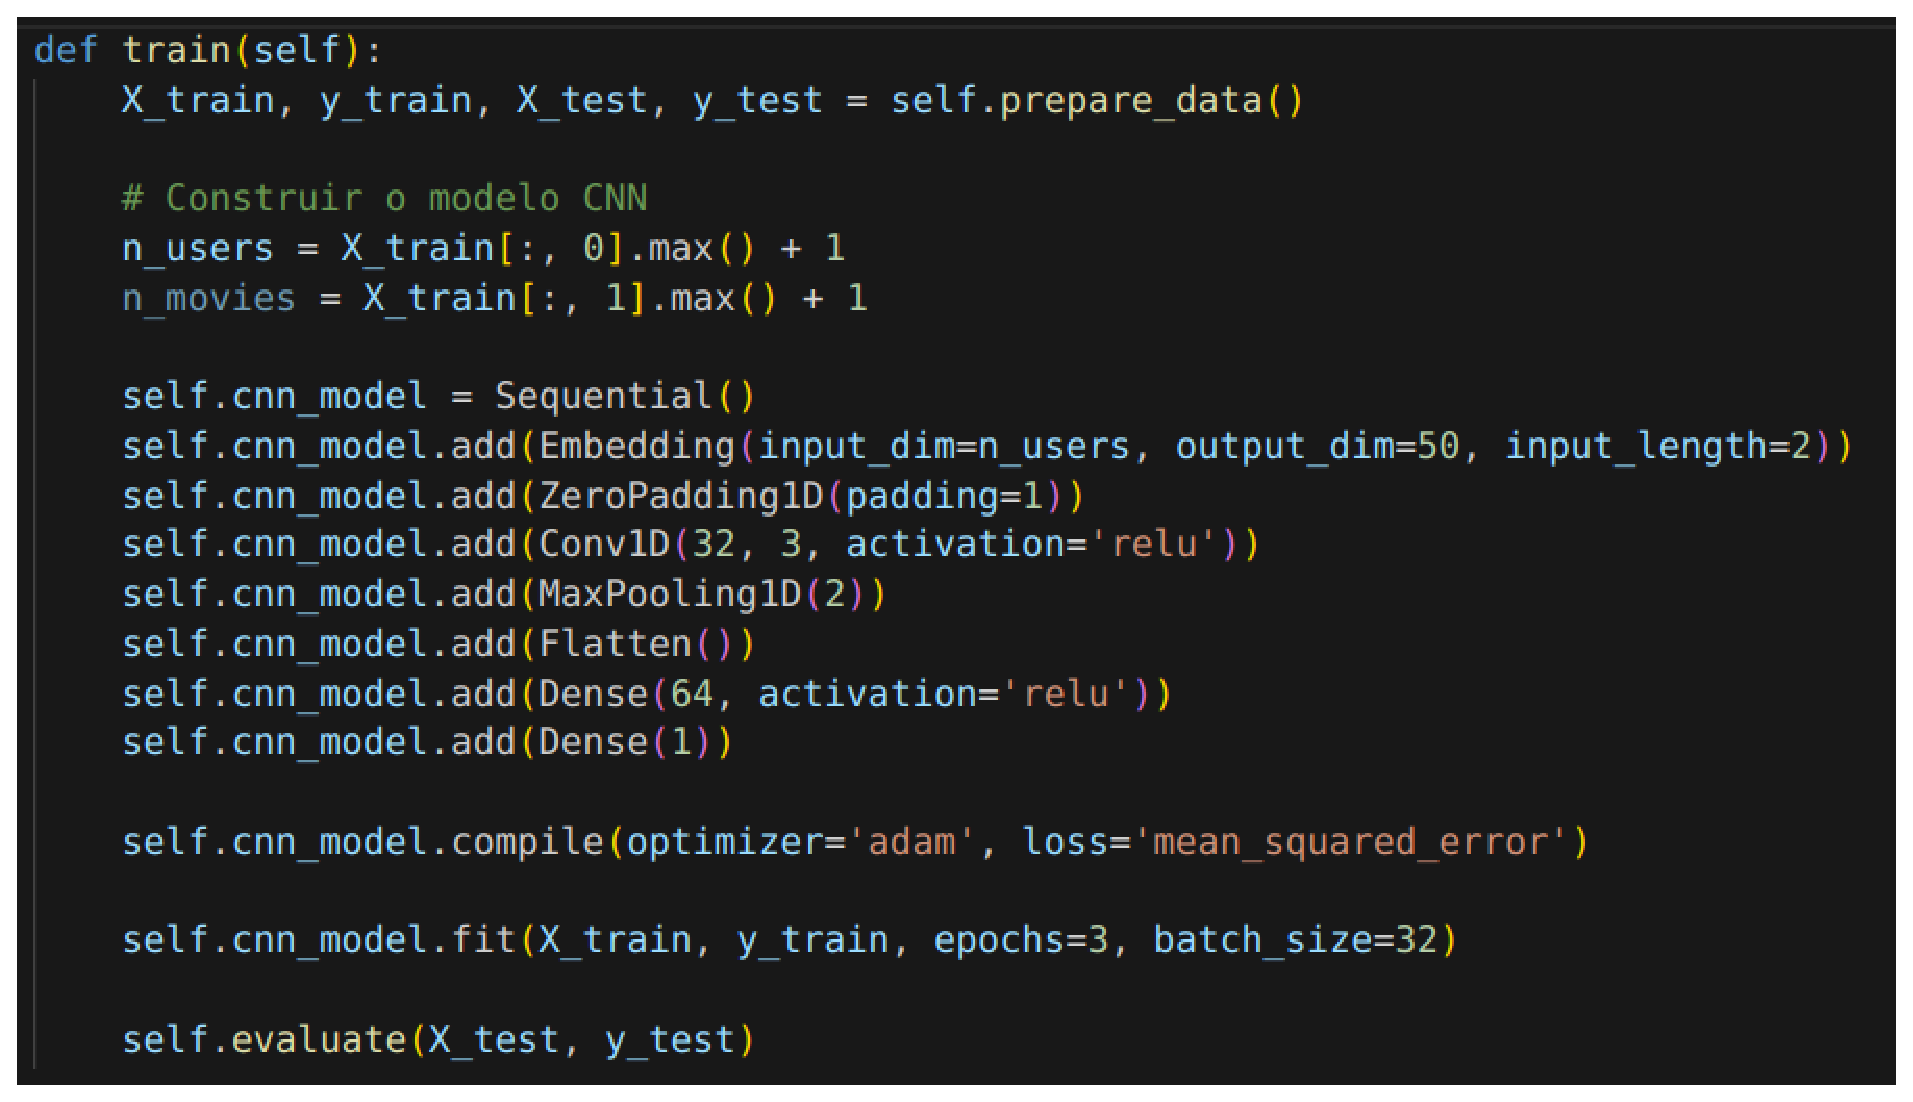
\includegraphics[width=0.5\textwidth]{figuras/train-cnn.eps}
        
        \vspace{2pt} % Espaço vertical entre a imagem e a fonte da imagem
        
        \small Fonte: Autora
    \end{figure}

    \item Avaliar Modelo: Função principal, responsável por avaliar o modelo com base nas métricas definidas na Seção 
    \hyperref[sec:meteanresul]{Método de Coleta e Análise de Resultados - Capítulo 4}
    \hyperref[sec:meteanresul]{ - Metodologia} 
    (Precisão, Revocação, Erro Médio Absoluto, Erro Quadrático Médio da Raiz).
    Apresentado na Figura \hyperref[fig:evaluate-cnn]{29};
    \begin{figure}[htbp]
        \centering
        \caption{Avaliar Modelo - Rede Neural Convolucional}
        \label{fig:evaluate-cnn}
        
        \vspace{2pt} % Espaço vertical entre a legenda e a imagem
        
        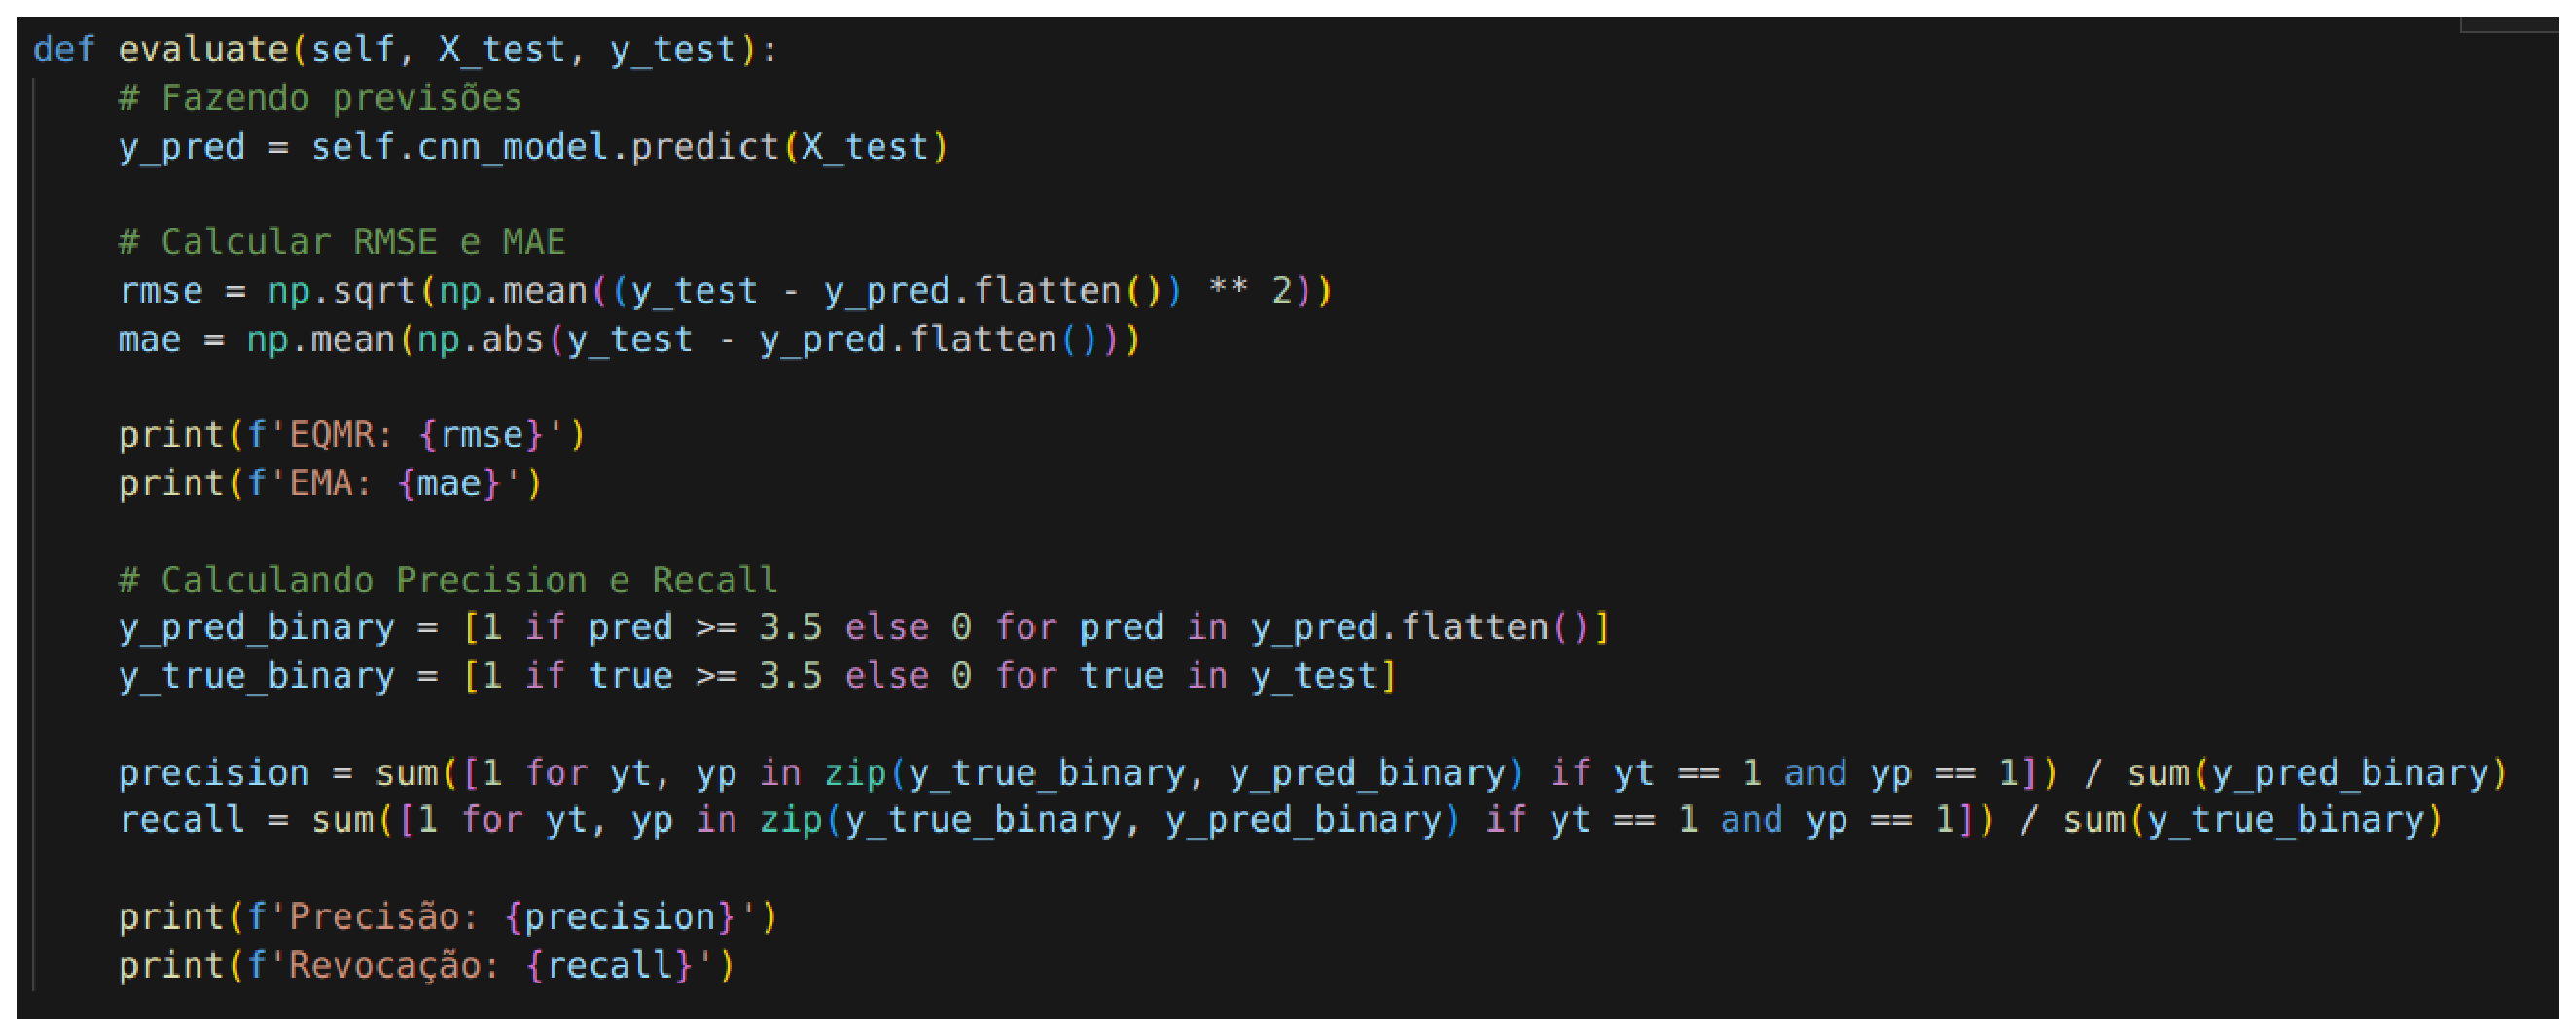
\includegraphics[width=0.5\textwidth]{figuras/evaluate-cnn.eps}
        
        \vspace{2pt} % Espaço vertical entre a imagem e a fonte da imagem
        
        \small Fonte: Autora
    \end{figure}

    \item Prever Avaliação: Função auxiliar, responsável por prever a avaliação do usuário para os filmes. Apresentado na
    Figura \hyperref[fig:pred-cnn]{30} e,
    \begin{figure}[htbp]
        \centering
        \caption{Prever Avaliação - Rede Neural Convolucional}
        \label{fig:pred-cnn}
        
        \vspace{2pt} % Espaço vertical entre a legenda e a imagem
        
        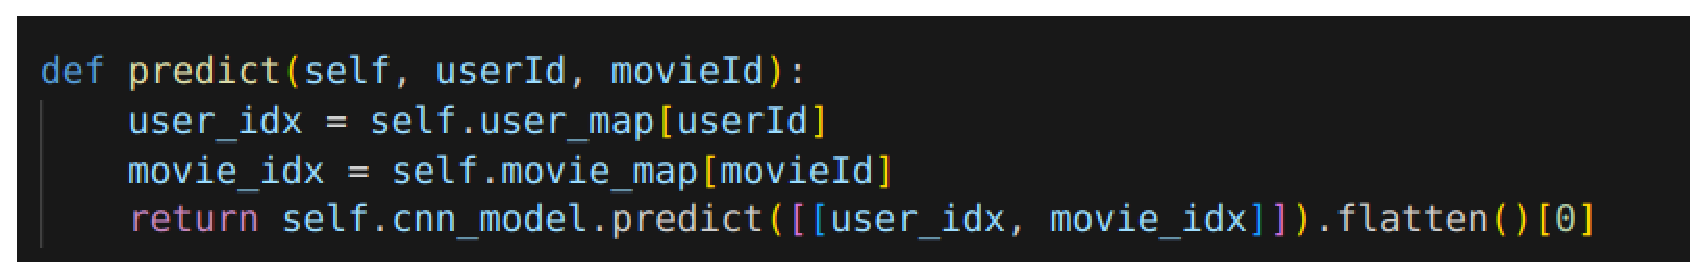
\includegraphics[width=0.5\textwidth]{figuras/pred-cnn.eps}
        
        \vspace{2pt} % Espaço vertical entre a imagem e a fonte da imagem
        
        \small Fonte: Autora
    \end{figure}

    \item Obter Recomendação: Função principal, responsável por recomendar ao usuário um filme. Apresentado na Figura
    \hyperref[fig:recomend-cnn]{31}.
    \begin{figure}[htbp]
        \centering
        \caption{Obter Recomendação - Rede Neural Convolucional}
        \label{fig:recomend-cnn}
        
        \vspace{2pt} % Espaço vertical entre a legenda e a imagem
        
        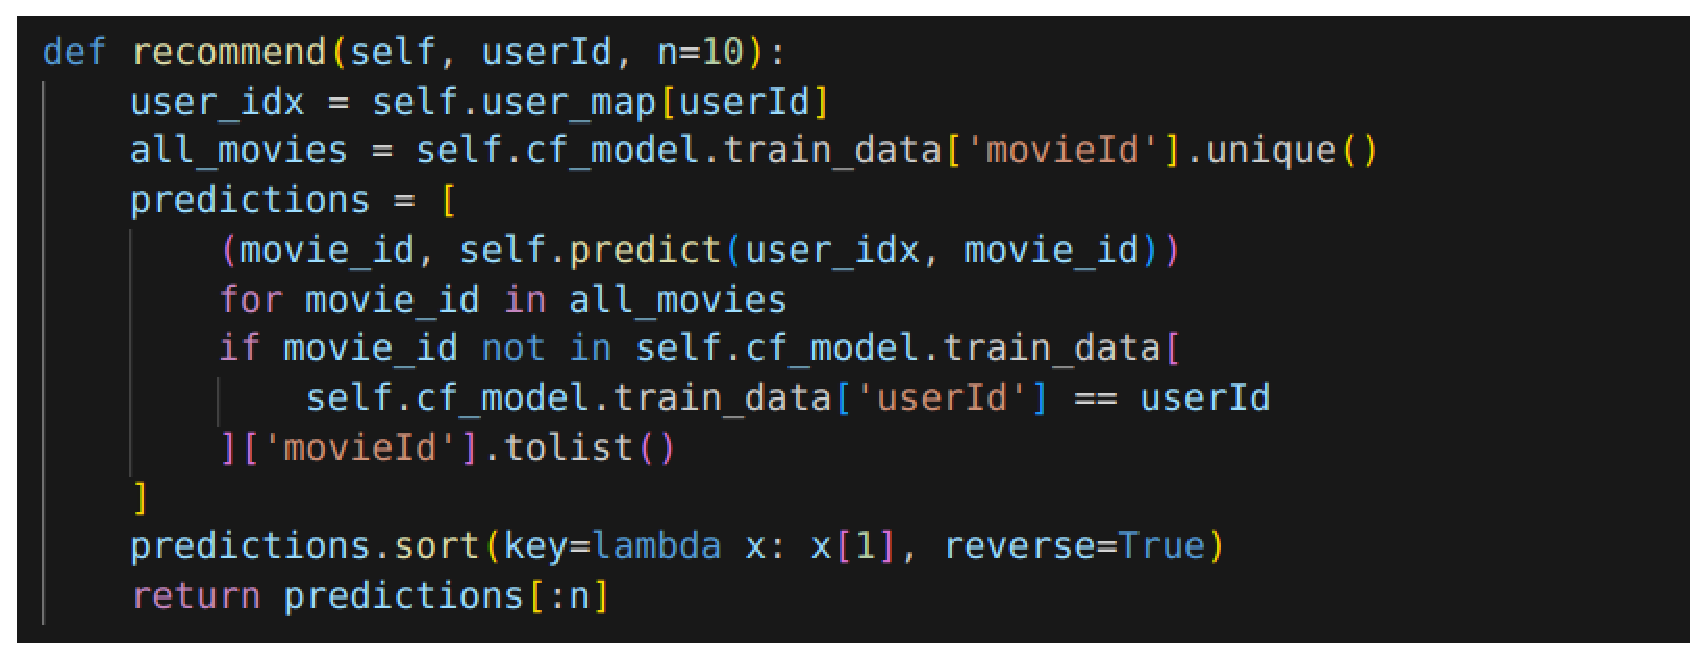
\includegraphics[width=0.5\textwidth]{figuras/recomend-cnn.eps}
        
        \vspace{2pt} % Espaço vertical entre a imagem e a fonte da imagem
        
        \small Fonte: Autora
    \end{figure}

\end{itemize}

Os resultados do modelo treinado por Redes Neurais Convolucionais é dado pela Figura \hyperref[fig:cnn-5]{32}:
\begin{figure}[htbp]
    \centering
    \caption{Resultados - Rede Neural Convolucional}
    \label{fig:cnn-5}
    
    \vspace{2pt} % Espaço vertical entre a legenda e a imagem
    
    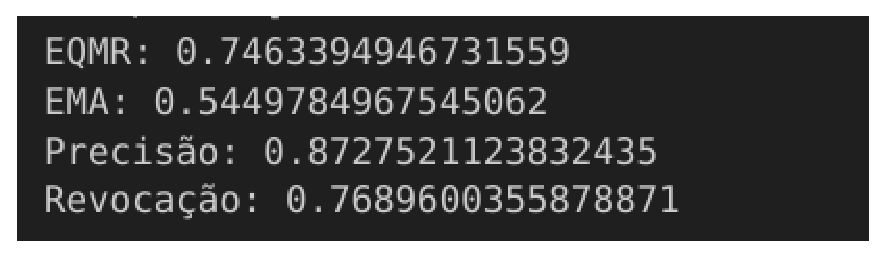
\includegraphics[width=0.5\textwidth]{figuras/cnn-5.eps}
    
    \vspace{2pt} % Espaço vertical entre a imagem e a fonte da imagem
    
    \small Fonte: Autora
\end{figure}

\subsection{Modelo com Redes Neurais Recorrentes}\label{subsec:rnr}

Usando como base o modelo de Filtros Colaborativos, por questão de memória do servidor do Colab, optou-se pela
versão que utiliza 5\%\ da base de dados.

Como nos outros modelos, no modelo com Redes Neurais Recorrentes, temos cinco funções, 
sendo três principais (treinar, avaliar, recomendar) e duas auxiliares (preparar base de dados, predizer).

\begin{itemize}
    \item Preparar Dados: Função auxiliar, responsável por carregar os dados da base de dados.
    Apresentado na Figura \hyperref[fig:prepdata-rnn]{33};
    \begin{figure}[htbp]
        \centering
        \caption{Preparar Dados - Rede Neural Recorrente}
        \label{fig:prepdata-rnn}
        
        \vspace{2pt} % Espaço vertical entre a legenda e a imagem
        
        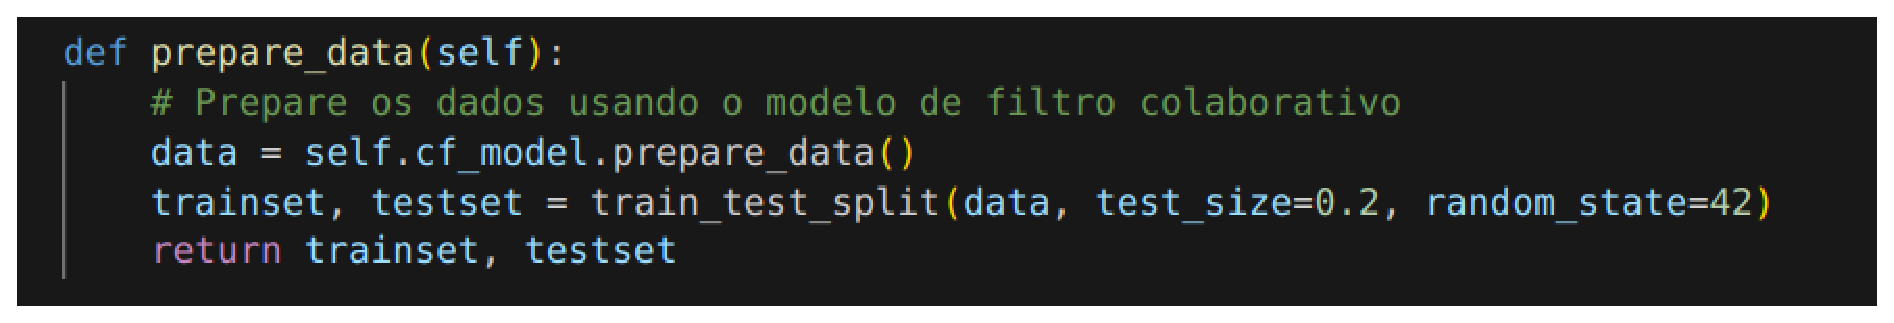
\includegraphics[width=0.5\textwidth]{figuras/prepdata-rnn.eps}
        
        \vspace{2pt} % Espaço vertical entre a imagem e a fonte da imagem
        
        \small Fonte: Autora
    \end{figure}

    \item Treinar Modelo: Função principal, responsável por treinar o modelo. Apresentado na Figura \hyperref[fig:train-rnn]{34};
    \begin{figure}[htbp]
        \centering
        \caption{Treinar Modelo - Rede Neural Recorrente}
        \label{fig:train-rnn}
        
        \vspace{2pt} % Espaço vertical entre a legenda e a imagem
        
        \includegraphics[width=0.5\textwidth]{figuras/train-rnn.eps}
        
        \vspace{2pt} % Espaço vertical entre a imagem e a fonte da imagem
        
        \small Fonte: Autora
    \end{figure}

    \item Avaliar Modelo: Função principal, responsável por avaliar o modelo com base nas métricas definidas na Seção 
    \hyperref[sec:meteanresul]{Método de Coleta e Análise de Resultados - Capítulo 4}
    \hyperref[sec:meteanresul]{ - Metodologia} 
    (Precisão, Revocação, Erro Médio Absoluto, Erro Quadrático Médio da Raiz).
    Apresentado na Figura \hyperref[fig:eval-rnn]{35};
    \begin{figure}[htbp]
        \centering
        \caption{Avaliar Modelo - Rede Neural Recorrente}
        \label{fig:eval-rnn}
        
        \vspace{2pt} % Espaço vertical entre a legenda e a imagem
        
        \includegraphics[width=0.5\textwidth]{figuras/eval-rnn.eps}
        
        \vspace{2pt} % Espaço vertical entre a imagem e a fonte da imagem
        
        \small Fonte: Autora
    \end{figure}

    \item Prever Avaliação: Função auxiliar, responsável por prever a avaliação do usuário para os filmes. Apresentado na
    Figura \hyperref[fig:pred-rnn]{36} e,
    \begin{figure}[htbp]
        \centering
        \caption{Prever Avaliação - Rede Neural Recorrente}
        \label{fig:pred-rnn}
        
        \vspace{2pt} % Espaço vertical entre a legenda e a imagem
        
        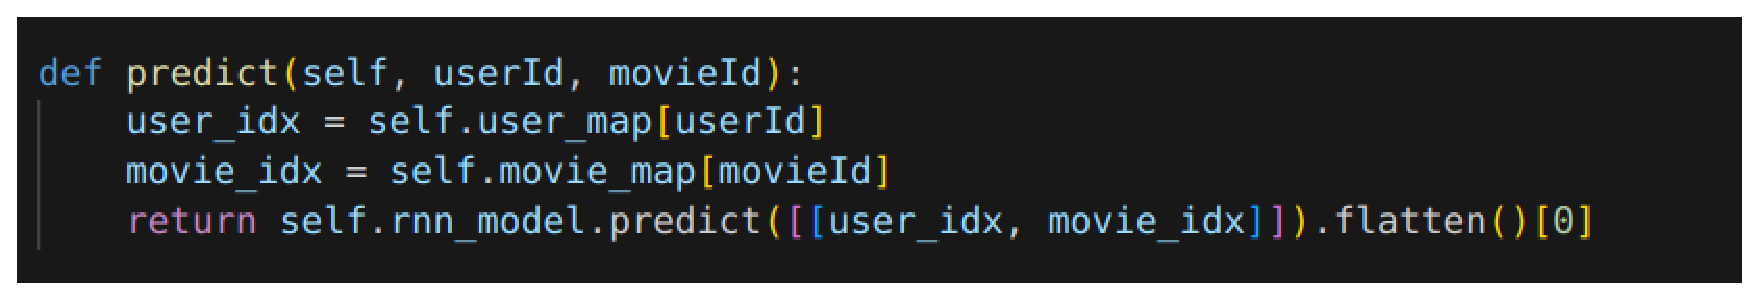
\includegraphics[width=0.5\textwidth]{figuras/pred-rnn.eps}
        
        \vspace{2pt} % Espaço vertical entre a imagem e a fonte da imagem
        
        \small Fonte: Autora
    \end{figure}

    \item Obter Recomendação: Função principal, responsável por recomendar ao usuário um filme. Apresentado na Figura
    \hyperref[fig:recom-rnn]{37}.
    \begin{figure}[htbp]
        \centering
        \caption{Obter Recomendação - Rede Neural Recorrente}
        \label{fig:recom-rnn}
        
        \vspace{2pt} % Espaço vertical entre a legenda e a imagem
        
        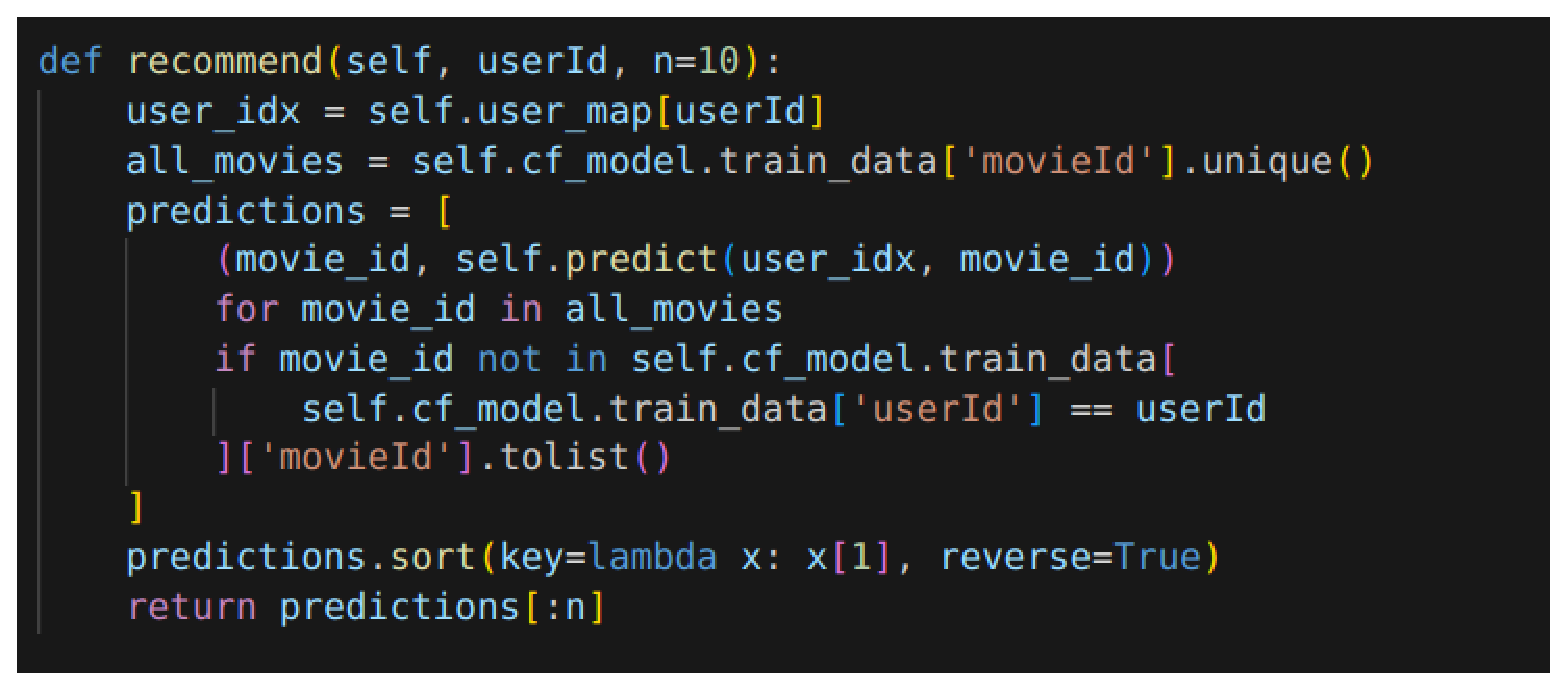
\includegraphics[width=0.5\textwidth]{figuras/recom-rnn.eps}
        
        \vspace{2pt} % Espaço vertical entre a imagem e a fonte da imagem
        
        \small Fonte: Autora
    \end{figure}

\end{itemize}

Os resultados do modelo treinado por Redes Neurais Recorrentes é dado pela Figura \hyperref[fig:rnn-5]{38}:
\begin{figure}[htbp]
    \centering
    \caption{Resultados - Rede Neural Recorrente}
    \label{fig:rnn-5}
    
    \vspace{2pt} % Espaço vertical entre a legenda e a imagem
    
    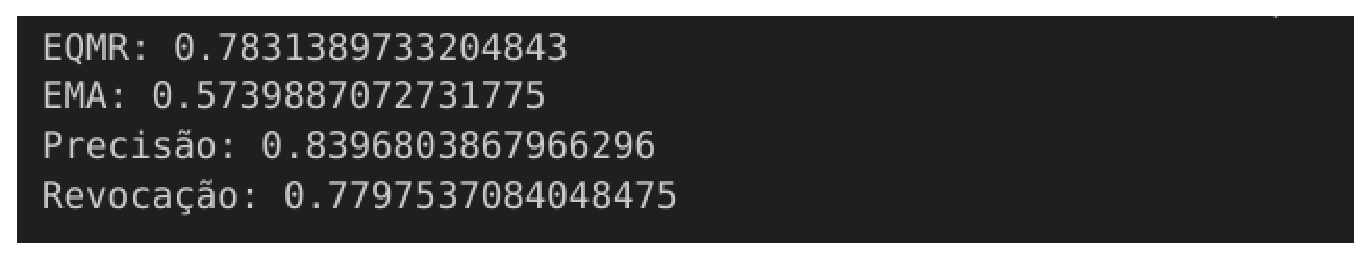
\includegraphics[width=0.5\textwidth]{figuras/rnn-5.eps}
    
    \vspace{2pt} % Espaço vertical entre a imagem e a fonte da imagem
    
    \small Fonte: Autora
\end{figure}

\subsection{Modelo com \textit{Autoencoder}}\label{subsec:autoencoder}

Usando como base o modelo de Filtros Colaborativos, por questão de memória do servidor do Colab, optou-se pela
versão que utiliza 5\%\ da base de dados.

Como nos outros modelos, no modelo com Autoencoder, temos cinco funções, 
sendo três principais (treinar, avaliar, recomendar) e duas auxiliares (preparar base de dados, predizer).

\begin{itemize}
    \item Preparar Dados: Função auxiliar, responsável por carregar e mapear os dados da base de dados.
    Apresentado na Figura \hyperref[fig:prepdata-aut]{39};
    \begin{figure}[htbp]
        \centering
        \caption{Preparar Dados - Autoencoder}
        \label{fig:prepdata-aut}
        
        \vspace{2pt} % Espaço vertical entre a legenda e a imagem
        
        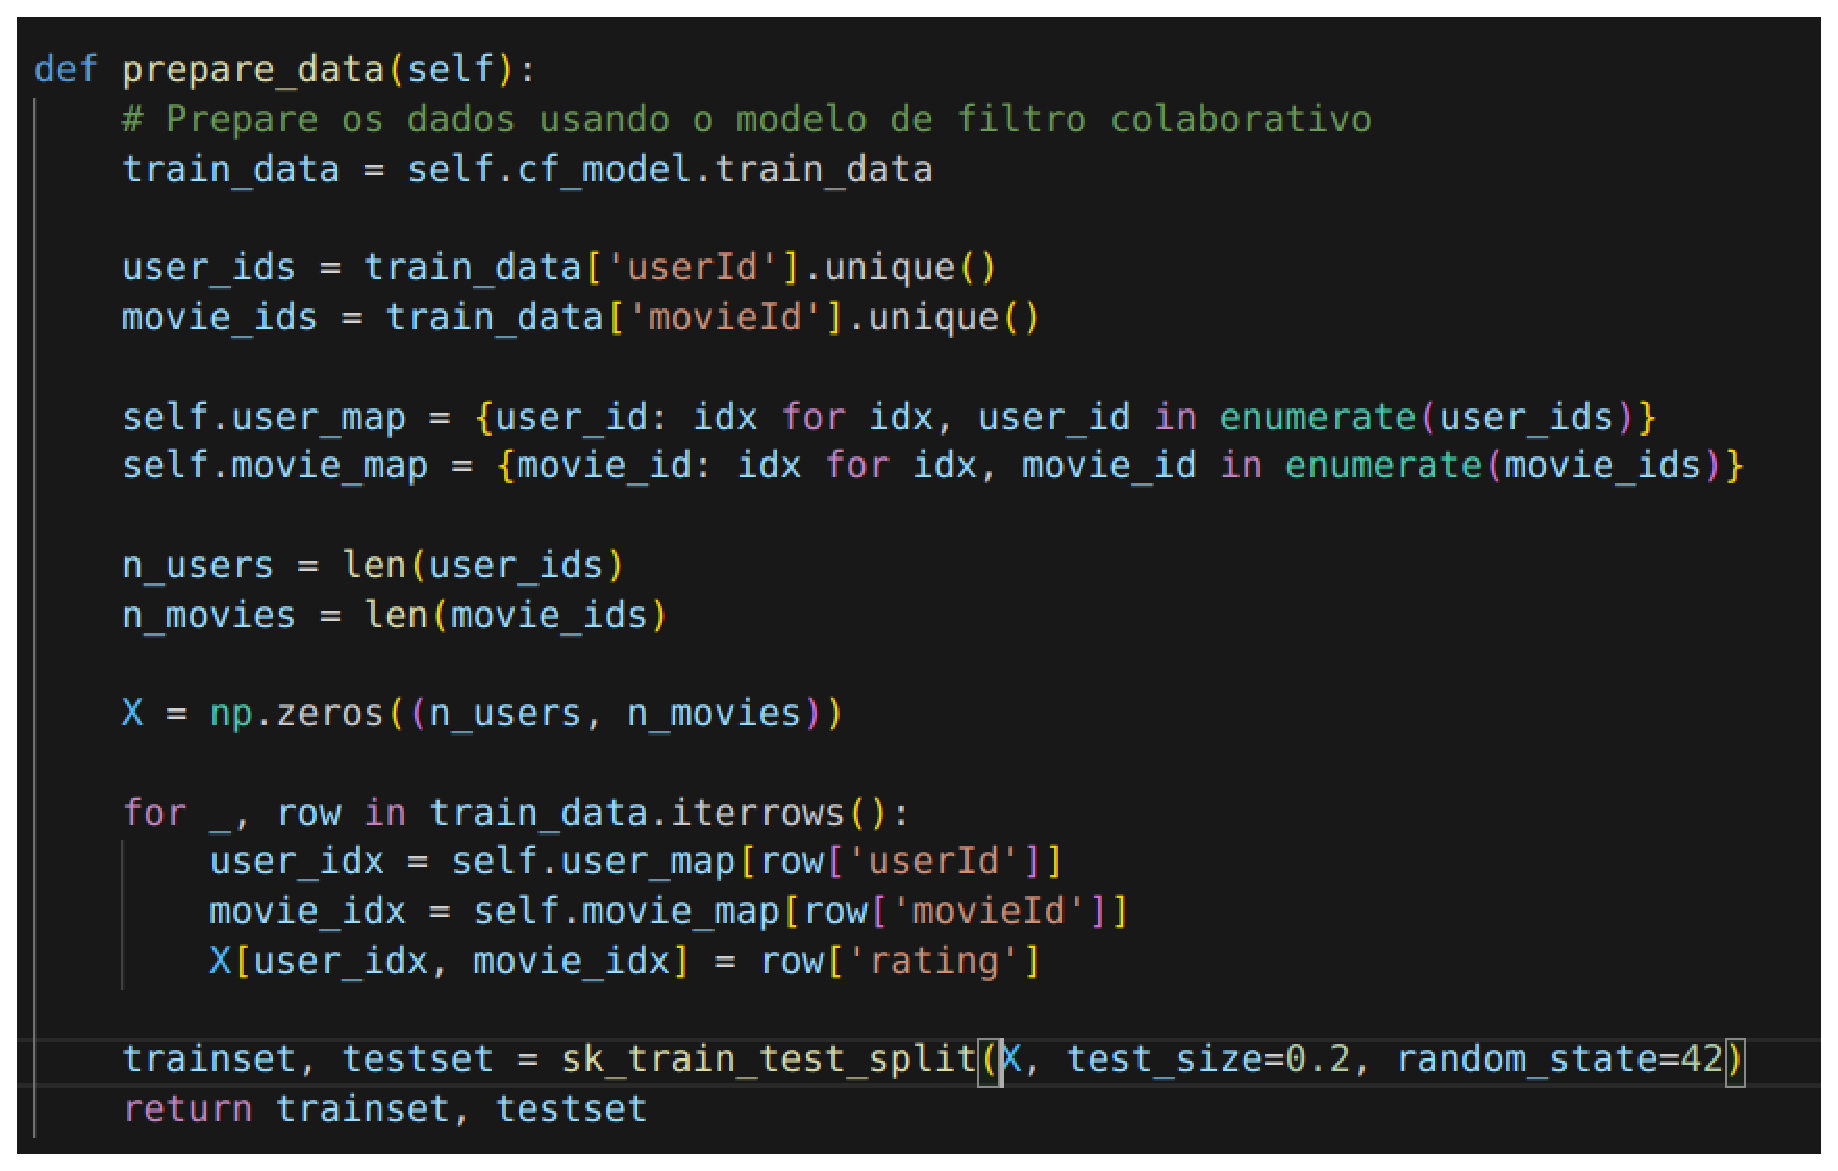
\includegraphics[width=0.5\textwidth]{figuras/prepdata-aut.eps}
        
        \vspace{2pt} % Espaço vertical entre a imagem e a fonte da imagem
        
        \small Fonte: Autora
    \end{figure}

    \item Treinar Modelo: Função principal, responsável por treinar o modelo. Apresentado na Figura \hyperref[fig:train-aut]{40};
    \begin{figure}[htbp]
        \centering
        \caption{Treinar Modelo - Autoencoder}
        \label{fig:train-aut}
        
        \vspace{2pt} % Espaço vertical entre a legenda e a imagem
        
        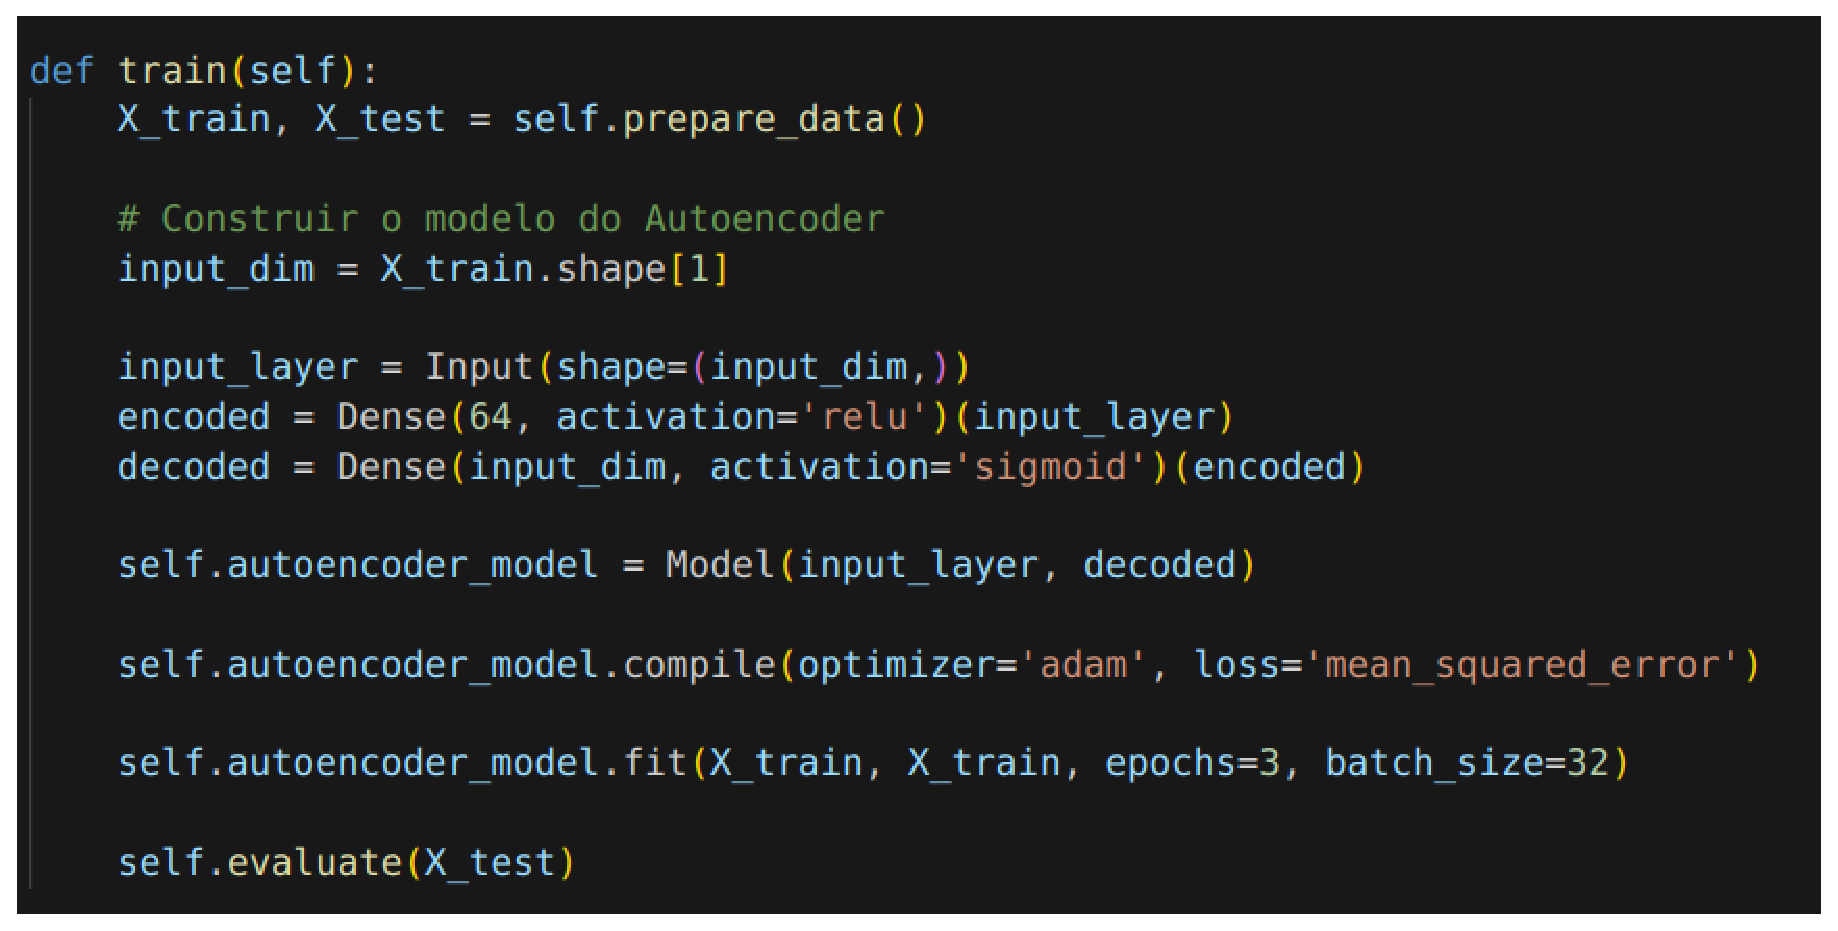
\includegraphics[width=0.5\textwidth]{figuras/train-aut.eps}
        
        \vspace{2pt} % Espaço vertical entre a imagem e a fonte da imagem
        
        \small Fonte: Autora
    \end{figure}

    \item Avaliar Modelo: Função principal, responsável por avaliar o modelo com base nas métricas definidas na Seção 
    \hyperref[sec:meteanresul]{Método de Coleta e Análise de Resultados - Capítulo 4}
    \hyperref[sec:meteanresul]{ - Metodologia} 
    (Precisão, Revocação, Erro Médio Absoluto, Erro Quadrático Médio da Raiz).
    Apresentado na Figura \hyperref[fig:eval-aut]{41};
    \begin{figure}[htbp]
        \centering
        \caption{Avaliar Modelo - Autoencoder}
        \label{fig:eval-aut}
        
        \vspace{2pt} % Espaço vertical entre a legenda e a imagem
        
        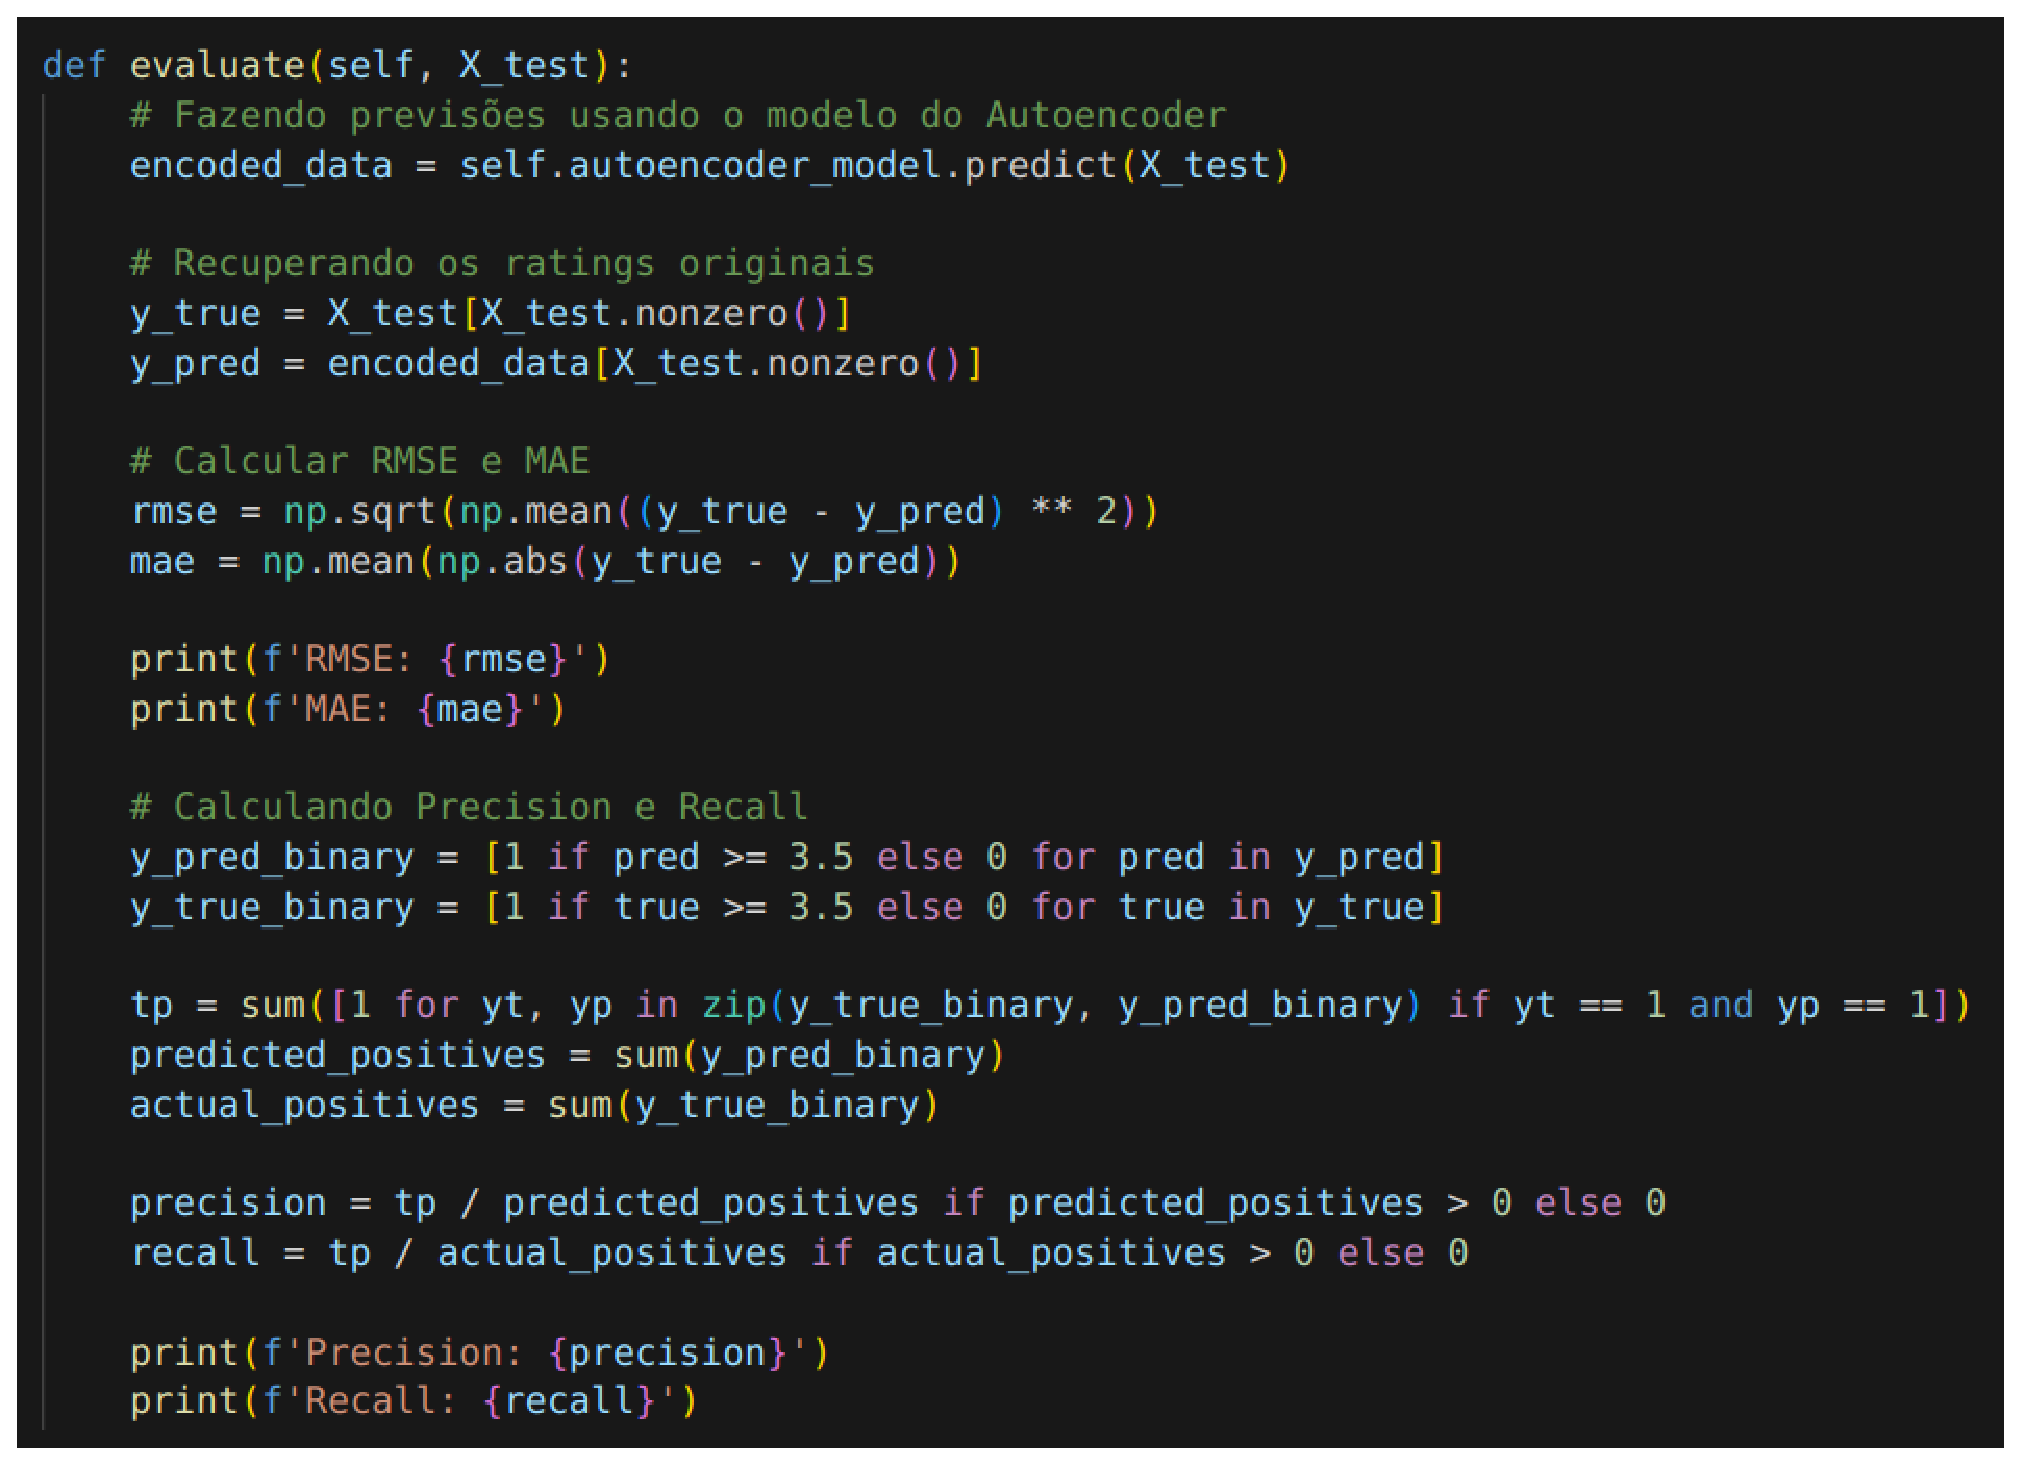
\includegraphics[width=0.5\textwidth]{figuras/eval-aut.eps}
        
        \vspace{2pt} % Espaço vertical entre a imagem e a fonte da imagem
        
        \small Fonte: Autora
    \end{figure}

    \item Prever Avaliação: Função auxiliar, responsável por prever a avaliação do usuário para os filmes. Apresentado na
    Figura \hyperref[fig:pred-aut]{42} e,
    \begin{figure}[htbp]
        \centering
        \caption{Prever Avaliação - Autoencoder}
        \label{fig:pred-aut}
        
        \vspace{2pt} % Espaço vertical entre a legenda e a imagem
        
        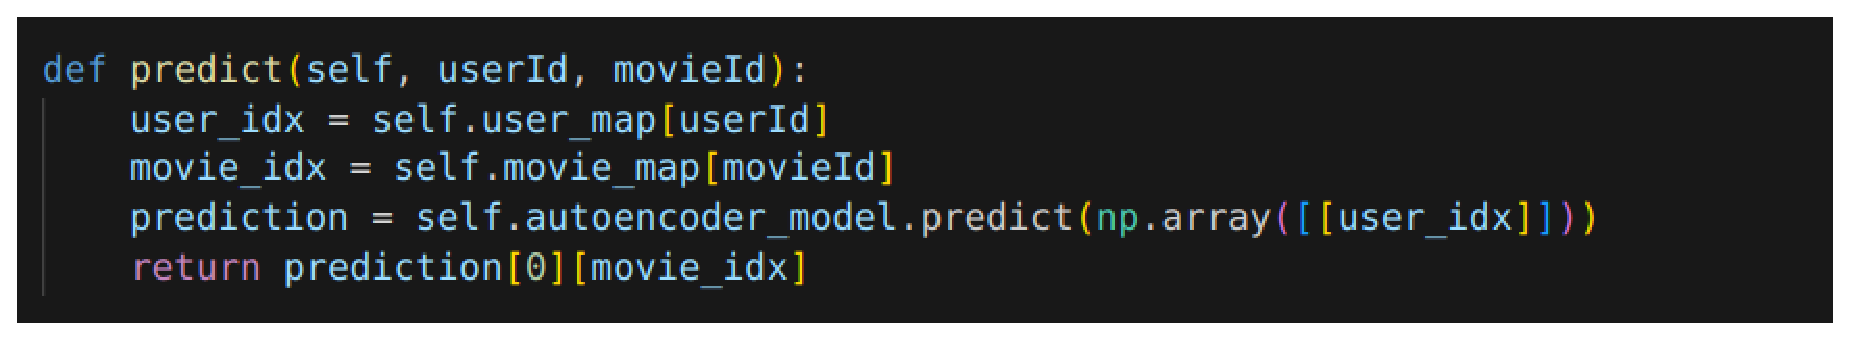
\includegraphics[width=0.5\textwidth]{figuras/pred-aut.eps}
        
        \vspace{2pt} % Espaço vertical entre a imagem e a fonte da imagem
        
        \small Fonte: Autora
    \end{figure}

    \item Obter Recomendação: Função principal, responsável por recomendar ao usuário um filme. Apresentado na Figura
    \hyperref[fig:recom-aut]{43}.
    \begin{figure}[htbp]
        \centering
        \caption{Obter Recomendação - Autoencoder}
        \label{fig:recom-aut}
        
        \vspace{2pt} % Espaço vertical entre a legenda e a imagem
        
        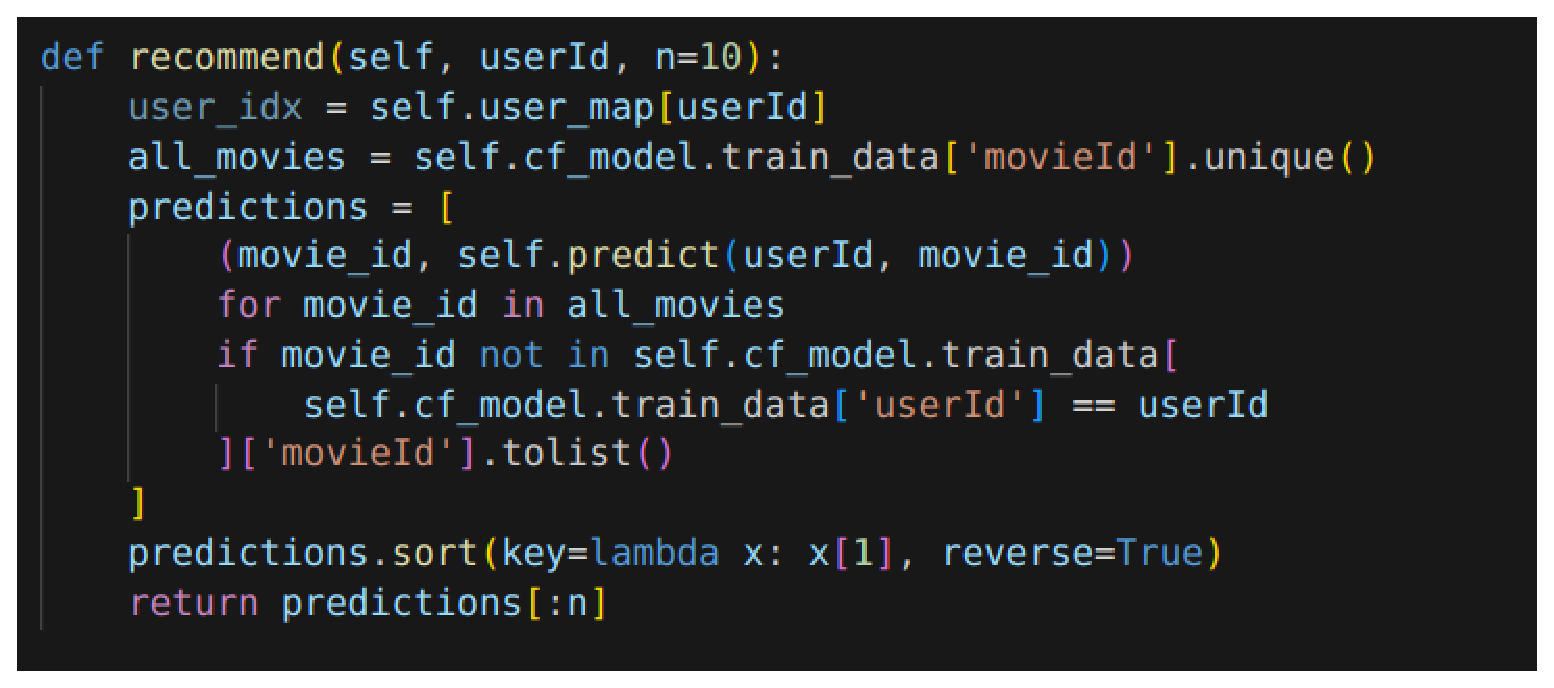
\includegraphics[width=0.5\textwidth]{figuras/recom-aut.eps}
        
        \vspace{2pt} % Espaço vertical entre a imagem e a fonte da imagem
        
        \small Fonte: Autora
    \end{figure}

\end{itemize}

Os resultados do modelo treinado por Redes Neurais Recorrentes é dado pela Figura \hyperref[fig:aut-5]{44}:
\begin{figure}[htbp]
    \centering
    \caption{Resultados - Autoencoder}
    \label{fig:aut-5}
    
    \vspace{2pt} % Espaço vertical entre a legenda e a imagem
    
    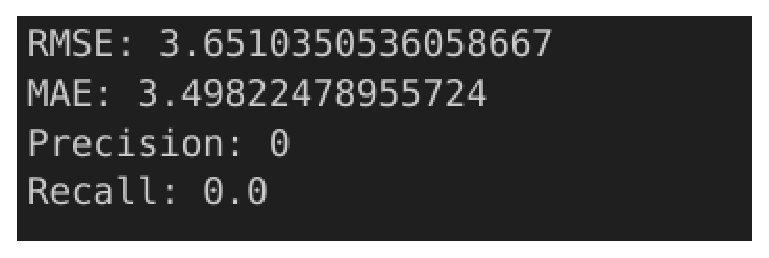
\includegraphics[width=0.5\textwidth]{figuras/aut-5.eps}
    
    \vspace{2pt} % Espaço vertical entre a imagem e a fonte da imagem
    
    \small Fonte: Autora
\end{figure}

Pode-se perceber que para o Autoencoder a Previsão e a Revocação são iguais a zero, isso ocorre porque como média
de avaliação foi definido o valor 3.5 (de 0 a 5), sendo acima de 3.5 considerado positivo e que seria item interessante
para o usuário. Já abaixo de 3.5, seriam itens que o usuário teria pouco ou nenhum interesse. Com ambos os valores zerados,
indica que nenhuma das previsões foi considerada positiva (>= 3.5). Além disso os valores de EQMR e EMA, divergem
bastante dos valores dos outros modelos (que estavam na casa do 0,7 e 0,5, respectivamente). Dessa forma, a solução
aplicando Autoencoder nos Filtros Colaborativos não pode ser considerada satisfatória.

\section{Solução Proposta para Sistema de Recomendação}\label{sec:solucao}

Comparando os modelos desenvolvidos e testados na Seção anterior, com base nas métricas e interpretações definidas
na Seção \hyperref[sec:meteanresul]{Método de Coleta e Análise de Resultados} \hyperref[sec:meteanresul]{ - Capítulo 4 - Metodologia}, o modelo que
apresenta as melhores métricas ao ser aplicado nos Filtros Colaborativos é o modelo de Rede Neural Convolucional. Portanto,
sendo o modelo a ser desenvolvido como proposta para este trabalho. Esse modelo em seguida será aplicado em uma \textit{API}, 
e apresentada aos usuários para validação. Em seguida, será coletado atráves de questionário, como apresentado na Seção
\hyperref[sec:meteanresul]{Método de Coleta e Análise de } \hyperref[sec:meteanresul]{ Resultados - Capítulo 4 - Metodologia}, e as respostas desse questionário
serão usadas para incrementar a base de dados e retreinar o modelo. Para, por fim, apresentar novamente ao usuário e reaplicar
o questionário, verificando se houve melhoria nas recomendações para aqueles usuários. 

\subsection{Filtros Colaborativos e \textit{Deep Learning}}\label{subsec:modelos}
Para a Solução Proposta para Sistema de Recomendação, será utilizado uma base de dados maior que a base
proposta durante as Provas de Conceito, ainda abordando a temática de recomendações voltadas para filmes. Como será utilizado
Filtros Colaborativos e Rede Neural Convolucional, ainda teremos o problema de "partida à frio". Assim, será acrescentado ao
modelo já desenvolvido durante as provas de conceito, uma lógica para lidar com esse problema, visto que os usuários da aplicação
ainda não possuem dados na base.

\subsection{API}\label{subsec:api}
Será desenvolvido uma aplicação \textit{web}, com base em um protótipo de alta fidelidade (ainda a ser desenvolvido),
que se integra com uma \textit{API} com o modelo de Rede Neural Convolucional com Filtros Colaborativos aplicado, e que 
retorna ao usuário recomendações de filmes com base no seu perfil.

\section{Resumo do Capítulo}\label{sec:resprop}
Este Capítulo aborda o contexto que a proposta deste trabalho surgiu, bem como a Solução Atual. A qual consiste em um conjunto
de testes com diferentes abordagens de Filtros e seus resultados, escolhendo o modelo que teve melhores métricas 
(Rede Neural Convolucional com Filtros Colaborativos). Além de apresentar qual seria a Solução Proposta deste Trabalho:
Uma aplicação que gera recomendações de filmes com base no perfil do usuário, e que utiliza o modelo de \textit{Deep Learning}
escolhido.